\documentclass[a4paper]{book}
\usepackage{a4wide}
\usepackage{makeidx}
\usepackage{fancyhdr}
\usepackage{graphicx}
\usepackage{multicol}
\usepackage{float}
\usepackage{textcomp}
\usepackage{alltt}
\usepackage{doxygen}
\makeindex
\setcounter{tocdepth}{1}
\renewcommand{\footrulewidth}{0.4pt}
\begin{document}
\begin{titlepage}
\vspace*{7cm}
\begin{center}
{\Large Reference Manual}\\
\vspace*{1cm}
{\large Generated by Doxygen 1.4.3}\\
\vspace*{0.5cm}
{\small �� 31. ��� 22:08:24 2007}\\
\end{center}
\end{titlepage}
\clearemptydoublepage
\pagenumbering{roman}
\tableofcontents
\clearemptydoublepage
\pagenumbering{arabic}
\chapter{Hierarchical Index}
\section{Class Hierarchy}
This inheritance list is sorted roughly, but not completely, alphabetically:\begin{CompactList}
\item \contentsline{section}{bbox}{\pageref{classbbox}}{}
\item \contentsline{section}{bounding\_\-box}{\pageref{classbounding__box}}{}
\item \contentsline{section}{cb\_\-intersection}{\pageref{structcb__intersection}}{}
\item \contentsline{section}{Cluster}{\pageref{struct_cluster}}{}
\item \contentsline{section}{color\_\-type}{\pageref{structcolor__type}}{}
\item \contentsline{section}{coord}{\pageref{structcoord}}{}
\item \contentsline{section}{Coord\_\-compare}{\pageref{struct_coord__compare}}{}
\item \contentsline{section}{coord\_\-type}{\pageref{structcoord__type}}{}
\item \contentsline{section}{correlation}{\pageref{structcorrelation}}{}
\item \contentsline{section}{edge\_\-cmp}{\pageref{classedge__cmp}}{}
\item \contentsline{section}{Expr}{\pageref{class_expr}}{}
\item \contentsline{section}{Field}{\pageref{struct_field}}{}
\item \contentsline{section}{geom\_\-grid}{\pageref{classgeom__grid}}{}
\item \contentsline{section}{geom\_\-grid::field\_\-struct}{\pageref{structgeom__grid_1_1field__struct}}{}
\item \contentsline{section}{Geophysics}{\pageref{struct_geophysics}}{}
\item \contentsline{section}{glyph\_\-type}{\pageref{structglyph__type}}{}
\item \contentsline{section}{grid\_\-type}{\pageref{structgrid__type}}{}
\item \contentsline{section}{gs\_\-lexord}{\pageref{classgs__lexord}}{}
\item \contentsline{section}{gs\_\-polord}{\pageref{classgs__polord}}{}
\item \contentsline{section}{hull\_\-type}{\pageref{structhull__type}}{}
\item \contentsline{section}{label\_\-site}{\pageref{structlabel__site}}{}
\item \contentsline{section}{Label\-Problem}{\pageref{struct_label_problem}}{}
\item \contentsline{section}{Label\-Site}{\pageref{struct_label_site}}{}
\item \contentsline{section}{lexord\_\-cmp}{\pageref{classlexord__cmp}}{}
\item \contentsline{section}{noddle\_\-type}{\pageref{structnoddle__type}}{}
\item \contentsline{section}{Node}{\pageref{union_node}}{}
\item \contentsline{section}{node\_\-func}{\pageref{classnode__func}}{}
\begin{CompactList}
\item \contentsline{section}{half\_\-space}{\pageref{classhalf__space}}{}
\end{CompactList}
\item \contentsline{section}{Number}{\pageref{struct_number}}{}
\item \contentsline{section}{Oper}{\pageref{struct_oper}}{}
\item \contentsline{section}{pgn\_\-builder}{\pageref{structpgn__builder}}{}
\begin{CompactList}
\item \contentsline{section}{back\_\-polygon}{\pageref{classback__polygon}}{}
\item \contentsline{section}{clip\_\-polygon}{\pageref{classclip__polygon}}{}
\end{CompactList}
\item \contentsline{section}{polygon\_\-grid}{\pageref{classpolygon__grid}}{}
\item \contentsline{section}{psstream}{\pageref{classpsstream}}{}
\item \contentsline{section}{psstream::Scale}{\pageref{structpsstream_1_1_scale}}{}
\item \contentsline{section}{psstream\_\-impl}{\pageref{classpsstream__impl}}{}
\item \contentsline{section}{quant}{\pageref{classquant}}{}
\item \contentsline{section}{s\_\-curve}{\pageref{classs__curve}}{}
\item \contentsline{section}{Sample}{\pageref{struct_sample}}{}
\item \contentsline{section}{Segment}{\pageref{struct_segment}}{}
\item \contentsline{section}{seqgen}{\pageref{classseqgen}}{}
\item \contentsline{section}{SH\_\-zero\_\-compare}{\pageref{class_s_h__zero__compare}}{}
\item \contentsline{section}{shape\_\-curve}{\pageref{structshape__curve}}{}
\item \contentsline{section}{shape\_\-type}{\pageref{structshape__type}}{}
\item \contentsline{section}{simplex}{\pageref{structsimplex}}{}
\item \contentsline{section}{Traj}{\pageref{struct_traj}}{}
\item \contentsline{section}{vertex\_\-compare}{\pageref{classvertex__compare}}{}
\item \contentsline{section}{Well}{\pageref{struct_well}}{}
\item \contentsline{section}{well\_\-grid}{\pageref{classwell__grid}}{}
\item \contentsline{section}{well\_\-grid\_\-key}{\pageref{structwell__grid__key}}{}
\item \contentsline{section}{well\_\-point\_\-set}{\pageref{classwell__point__set}}{}
\item \contentsline{section}{well\_\-type}{\pageref{structwell__type}}{}
\item \contentsline{section}{wg\_\-wrapper}{\pageref{classwg__wrapper}}{}
\item \contentsline{section}{yyalloc}{\pageref{unionyyalloc}}{}
\item \contentsline{section}{Zero\_\-type}{\pageref{struct_zero__type}}{}
\end{CompactList}

\chapter{Class Index}
\section{Class List}
Here are the classes, structs, unions and interfaces with brief descriptions:\begin{CompactList}
\item\contentsline{section}{{\bf back\_\-polygon} }{\pageref{classback__polygon}}{}
\item\contentsline{section}{{\bf bbox} }{\pageref{classbbox}}{}
\item\contentsline{section}{{\bf bounding\_\-box} }{\pageref{classbounding__box}}{}
\item\contentsline{section}{{\bf cb\_\-intersection} }{\pageref{structcb__intersection}}{}
\item\contentsline{section}{{\bf clip\_\-polygon} }{\pageref{classclip__polygon}}{}
\item\contentsline{section}{{\bf Cluster} }{\pageref{struct_cluster}}{}
\item\contentsline{section}{{\bf color\_\-type} }{\pageref{structcolor__type}}{}
\item\contentsline{section}{{\bf coord} }{\pageref{structcoord}}{}
\item\contentsline{section}{{\bf Coord\_\-compare} }{\pageref{struct_coord__compare}}{}
\item\contentsline{section}{{\bf coord\_\-type} }{\pageref{structcoord__type}}{}
\item\contentsline{section}{{\bf correlation} }{\pageref{structcorrelation}}{}
\item\contentsline{section}{{\bf edge\_\-cmp} }{\pageref{classedge__cmp}}{}
\item\contentsline{section}{{\bf Expr} }{\pageref{class_expr}}{}
\item\contentsline{section}{{\bf Field} }{\pageref{struct_field}}{}
\item\contentsline{section}{{\bf geom\_\-grid} }{\pageref{classgeom__grid}}{}
\item\contentsline{section}{{\bf geom\_\-grid::field\_\-struct} }{\pageref{structgeom__grid_1_1field__struct}}{}
\item\contentsline{section}{{\bf Geophysics} }{\pageref{struct_geophysics}}{}
\item\contentsline{section}{{\bf glyph\_\-type} }{\pageref{structglyph__type}}{}
\item\contentsline{section}{{\bf grid\_\-type} }{\pageref{structgrid__type}}{}
\item\contentsline{section}{{\bf gs\_\-lexord} }{\pageref{classgs__lexord}}{}
\item\contentsline{section}{{\bf gs\_\-polord} }{\pageref{classgs__polord}}{}
\item\contentsline{section}{{\bf half\_\-space} }{\pageref{classhalf__space}}{}
\item\contentsline{section}{{\bf hull\_\-type} }{\pageref{structhull__type}}{}
\item\contentsline{section}{{\bf label\_\-site} }{\pageref{structlabel__site}}{}
\item\contentsline{section}{{\bf Label\-Problem} }{\pageref{struct_label_problem}}{}
\item\contentsline{section}{{\bf Label\-Site} }{\pageref{struct_label_site}}{}
\item\contentsline{section}{{\bf lexord\_\-cmp} }{\pageref{classlexord__cmp}}{}
\item\contentsline{section}{{\bf noddle\_\-type} }{\pageref{structnoddle__type}}{}
\item\contentsline{section}{{\bf Node} }{\pageref{union_node}}{}
\item\contentsline{section}{{\bf node\_\-func} }{\pageref{classnode__func}}{}
\item\contentsline{section}{{\bf Number} }{\pageref{struct_number}}{}
\item\contentsline{section}{{\bf Oper} }{\pageref{struct_oper}}{}
\item\contentsline{section}{{\bf pgn\_\-builder} }{\pageref{structpgn__builder}}{}
\item\contentsline{section}{{\bf polygon\_\-grid} }{\pageref{classpolygon__grid}}{}
\item\contentsline{section}{{\bf psstream} }{\pageref{classpsstream}}{}
\item\contentsline{section}{{\bf psstream::Scale} }{\pageref{structpsstream_1_1_scale}}{}
\item\contentsline{section}{{\bf psstream\_\-impl} }{\pageref{classpsstream__impl}}{}
\item\contentsline{section}{{\bf quant} }{\pageref{classquant}}{}
\item\contentsline{section}{{\bf s\_\-curve} }{\pageref{classs__curve}}{}
\item\contentsline{section}{{\bf Sample} }{\pageref{struct_sample}}{}
\item\contentsline{section}{{\bf Segment} }{\pageref{struct_segment}}{}
\item\contentsline{section}{{\bf seqgen} }{\pageref{classseqgen}}{}
\item\contentsline{section}{{\bf SH\_\-zero\_\-compare} }{\pageref{class_s_h__zero__compare}}{}
\item\contentsline{section}{{\bf shape\_\-curve} }{\pageref{structshape__curve}}{}
\item\contentsline{section}{{\bf shape\_\-type} }{\pageref{structshape__type}}{}
\item\contentsline{section}{{\bf simplex} }{\pageref{structsimplex}}{}
\item\contentsline{section}{{\bf Traj} }{\pageref{struct_traj}}{}
\item\contentsline{section}{{\bf vertex\_\-compare} }{\pageref{classvertex__compare}}{}
\item\contentsline{section}{{\bf Well} }{\pageref{struct_well}}{}
\item\contentsline{section}{{\bf well\_\-grid} }{\pageref{classwell__grid}}{}
\item\contentsline{section}{{\bf well\_\-grid\_\-key} }{\pageref{structwell__grid__key}}{}
\item\contentsline{section}{{\bf well\_\-point\_\-set} }{\pageref{classwell__point__set}}{}
\item\contentsline{section}{{\bf well\_\-type} }{\pageref{structwell__type}}{}
\item\contentsline{section}{{\bf wg\_\-wrapper} }{\pageref{classwg__wrapper}}{}
\item\contentsline{section}{{\bf yyalloc} }{\pageref{unionyyalloc}}{}
\item\contentsline{section}{{\bf Zero\_\-type} }{\pageref{struct_zero__type}}{}
\end{CompactList}

\chapter{Class Documentation}
\section{back\_\-polygon Class Reference}
\label{classback__polygon}\index{back_polygon@{back\_\-polygon}}
Inheritance diagram for back\_\-polygon:\begin{figure}[H]
\begin{center}
\leavevmode
\includegraphics[width=70pt]{classback__polygon__inherit__graph}
\end{center}
\end{figure}
Collaboration diagram for back\_\-polygon:\begin{figure}[H]
\begin{center}
\leavevmode
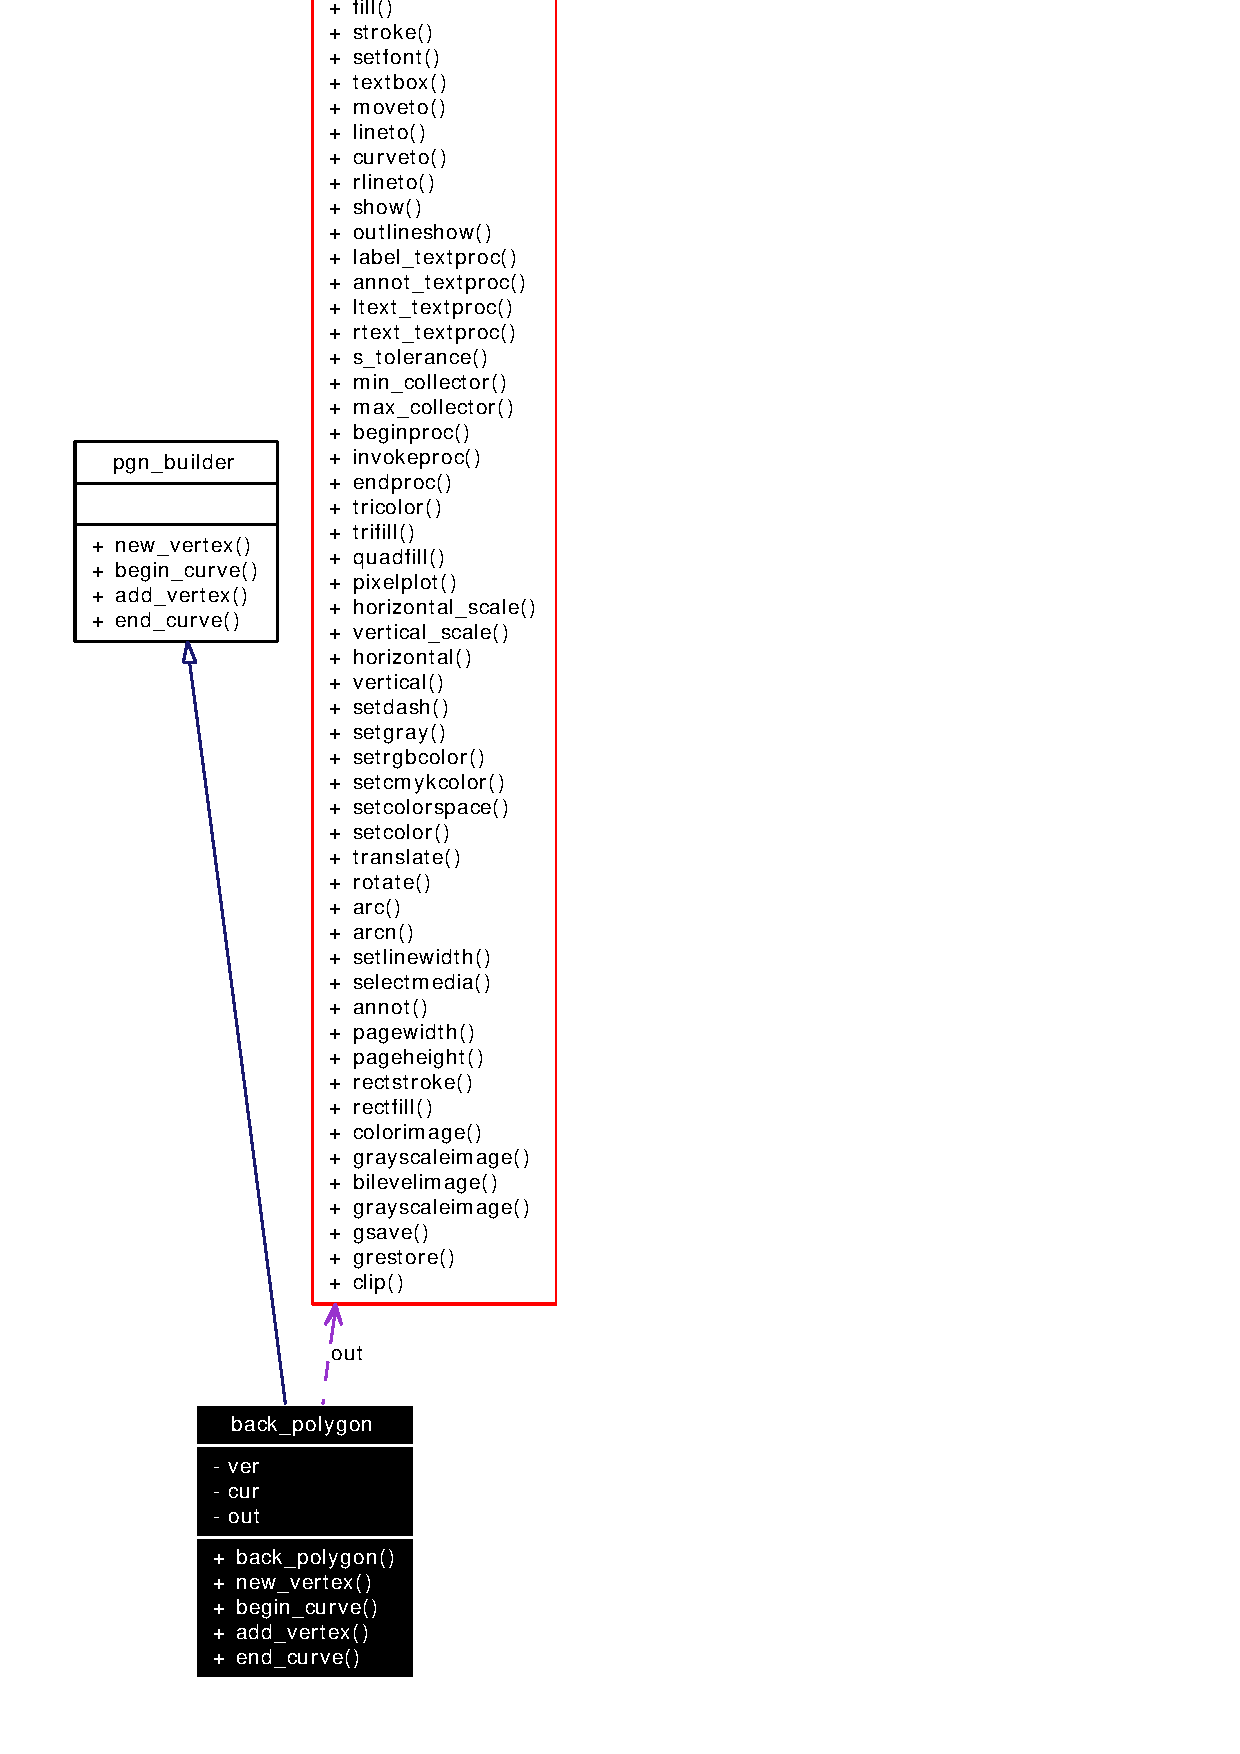
\includegraphics[width=133pt]{classback__polygon__coll__graph}
\end{center}
\end{figure}
\subsection*{Public Member Functions}
\begin{CompactItemize}
\item 
{\bf back\_\-polygon} ({\bf psstream} \&o)\label{classback__polygon_a0}

\item 
int {\bf new\_\-vertex} (double x, double y)\label{classback__polygon_a1}

\item 
void {\bf begin\_\-curve} ()\label{classback__polygon_a2}

\item 
void {\bf add\_\-vertex} (int)\label{classback__polygon_a3}

\item 
void {\bf end\_\-curve} ()\label{classback__polygon_a4}

\end{CompactItemize}


\subsection{Detailed Description}




Definition at line 227 of file ps\_\-data.h.

The documentation for this class was generated from the following files:\begin{CompactItemize}
\item 
ps\_\-data.h\item 
ps\_\-text.cpp\end{CompactItemize}

\section{bbox Class Reference}
\label{classbbox}\index{bbox@{bbox}}
Collaboration diagram for bbox:\begin{figure}[H]
\begin{center}
\leavevmode
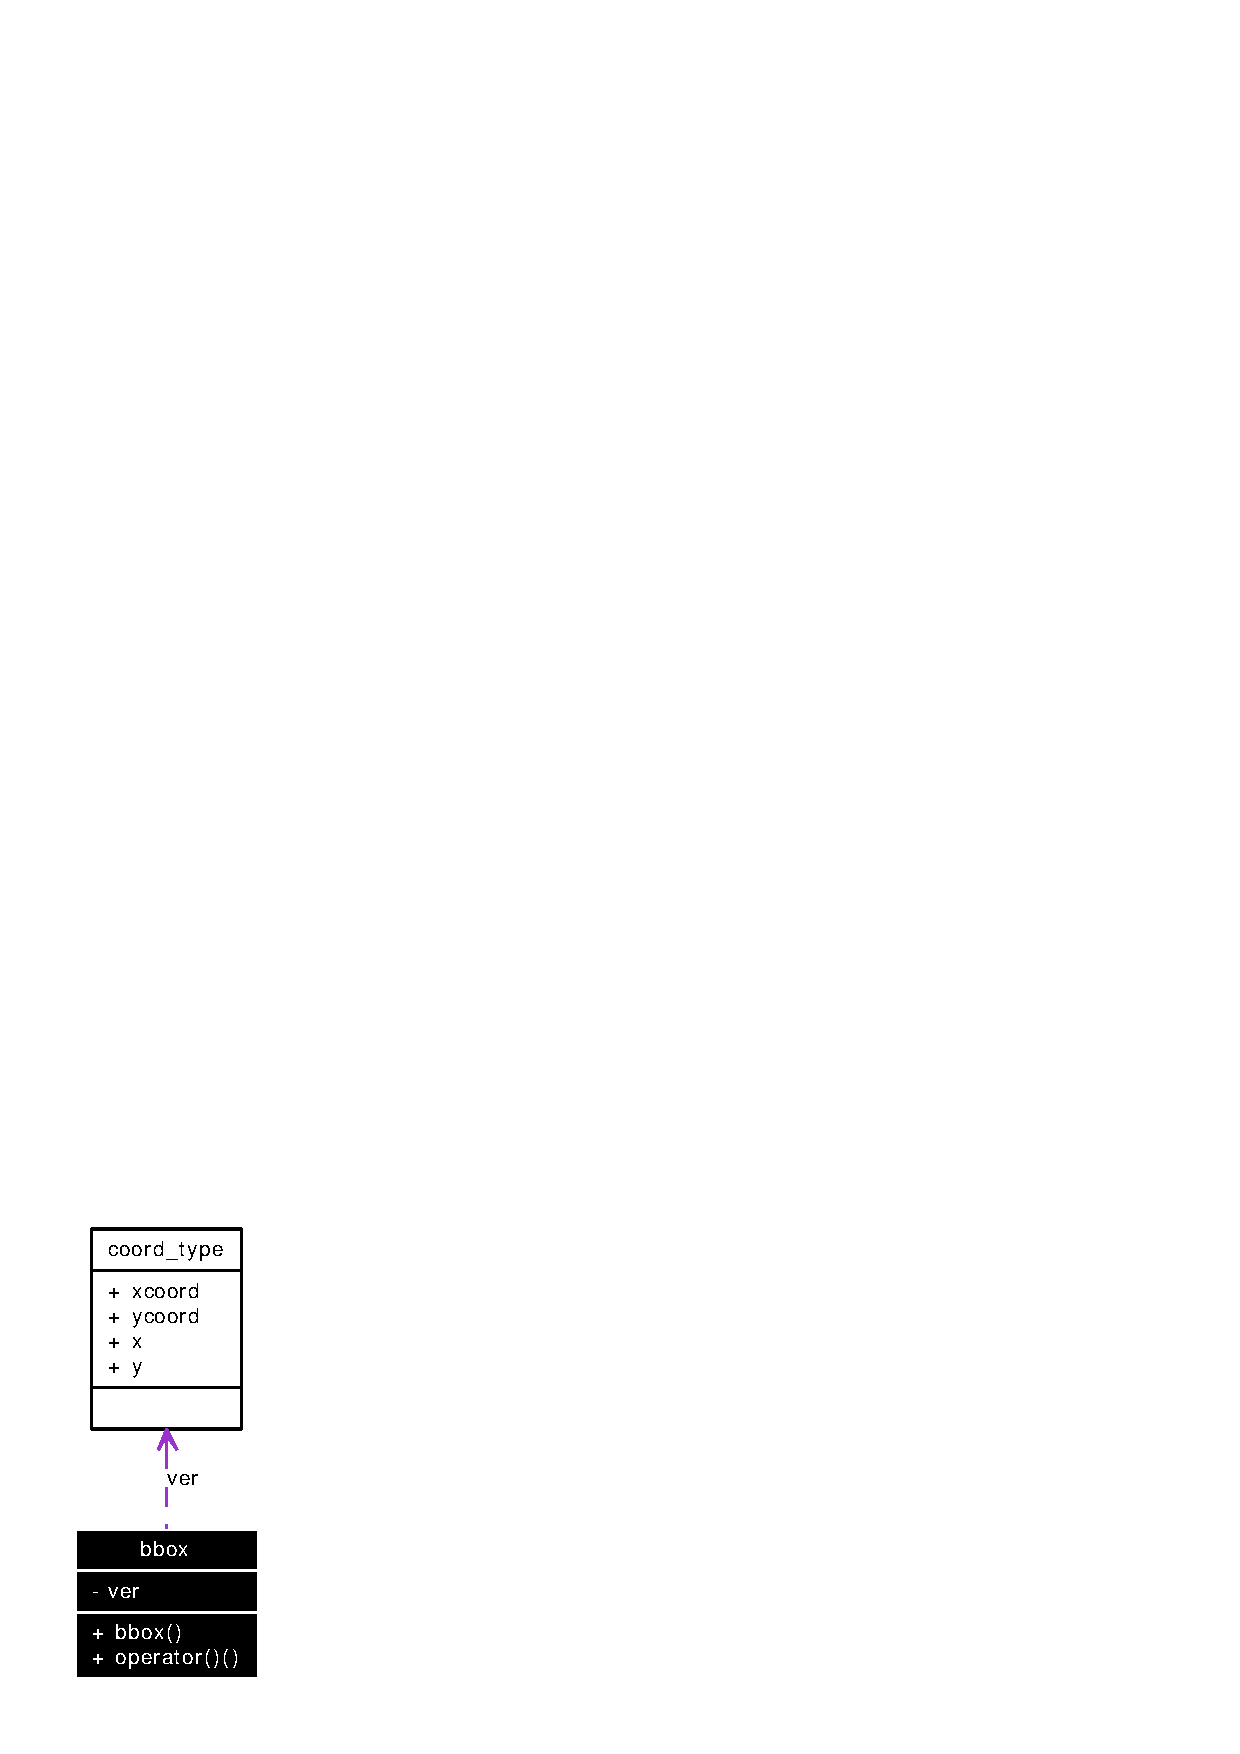
\includegraphics[width=62pt]{classbbox__coll__graph}
\end{center}
\end{figure}
\subsection*{Public Member Functions}
\begin{CompactItemize}
\item 
{\bf bbox} (const {\bf coord\_\-type} $\ast$p)\label{classbbox_a0}

\item 
double $\ast$ {\bf operator()} (double $\ast$bb, int n) const \label{classbbox_a1}

\end{CompactItemize}


\subsection{Detailed Description}




Definition at line 36 of file z2.cpp.

The documentation for this class was generated from the following file:\begin{CompactItemize}
\item 
z2.cpp\end{CompactItemize}

\section{bounding\_\-box Class Reference}
\label{classbounding__box}\index{bounding_box@{bounding\_\-box}}
Collaboration diagram for bounding\_\-box:\begin{figure}[H]
\begin{center}
\leavevmode
\includegraphics[width=71pt]{classbounding__box__coll__graph}
\end{center}
\end{figure}
\subsection*{Public Member Functions}
\begin{CompactItemize}
\item 
{\bf bounding\_\-box} (const {\bf coord\_\-type} $\ast$p)\label{classbounding__box_a0}

\item 
double $\ast$ {\bf operator()} (double $\ast$bb, int n) const \label{classbounding__box_a1}

\end{CompactItemize}
\subsection*{Static Public Member Functions}
\begin{CompactItemize}
\item 
static double $\ast$ {\bf max} (double $\ast$bb)\label{classbounding__box_e0}

\item 
static double $\ast$ {\bf init} (const {\bf coord\_\-type} \&p, double $\ast$bb)\label{classbounding__box_e1}

\end{CompactItemize}


\subsection{Detailed Description}




Definition at line 253 of file ps\_\-data.h.

The documentation for this class was generated from the following files:\begin{CompactItemize}
\item 
ps\_\-data.h\item 
ps\_\-bbox.cpp\end{CompactItemize}

\section{cb\_\-intersection Struct Reference}
\label{structcb__intersection}\index{cb_intersection@{cb\_\-intersection}}
\subsection*{Public Attributes}
\begin{CompactItemize}
\item 
int {\bf index}\label{structcb__intersection_o0}

\item 
bool {\bf entering}\label{structcb__intersection_o1}

\item 
double {\bf param}\label{structcb__intersection_o2}

\end{CompactItemize}


\subsection{Detailed Description}




Definition at line 789 of file ps\_\-clip.cpp.

The documentation for this struct was generated from the following file:\begin{CompactItemize}
\item 
ps\_\-clip.cpp\end{CompactItemize}

\section{clip\_\-polygon Class Reference}
\label{classclip__polygon}\index{clip_polygon@{clip\_\-polygon}}
Inheritance diagram for clip\_\-polygon:\begin{figure}[H]
\begin{center}
\leavevmode
\includegraphics[width=67pt]{classclip__polygon__inherit__graph}
\end{center}
\end{figure}
Collaboration diagram for clip\_\-polygon:\begin{figure}[H]
\begin{center}
\leavevmode
\includegraphics[width=67pt]{classclip__polygon__coll__graph}
\end{center}
\end{figure}
\subsection*{Public Member Functions}
\begin{CompactItemize}
\item 
{\bf clip\_\-polygon} (vertex\_\-type \&v, edge\_\-type \&e)\label{classclip__polygon_a0}

\item 
int {\bf new\_\-vertex} (double x, double y)\label{classclip__polygon_a1}

\item 
void {\bf begin\_\-curve} ()\label{classclip__polygon_a2}

\item 
void {\bf add\_\-vertex} (int)\label{classclip__polygon_a3}

\item 
void {\bf end\_\-curve} ()\label{classclip__polygon_a4}

\end{CompactItemize}


\subsection{Detailed Description}




Definition at line 240 of file ps\_\-data.h.

The documentation for this class was generated from the following files:\begin{CompactItemize}
\item 
ps\_\-data.h\item 
ps\_\-clip.cpp\end{CompactItemize}

\section{Cluster Struct Reference}
\label{struct_cluster}\index{Cluster@{Cluster}}
\subsection*{Public Attributes}
\begin{CompactItemize}
\item 
long {\bf number}\label{struct_cluster_o0}

\item 
char {\bf name} [6]\label{struct_cluster_o1}

\item 
float {\bf xcoord}\label{struct_cluster_o2}

\item 
float {\bf ycoord}\label{struct_cluster_o3}

\end{CompactItemize}


\subsection{Detailed Description}




Definition at line 63 of file surface\_\-pick.cpp.

The documentation for this struct was generated from the following file:\begin{CompactItemize}
\item 
surface\_\-pick.cpp\end{CompactItemize}

\section{color\_\-type Struct Reference}
\label{structcolor__type}\index{color_type@{color\_\-type}}
\subsection*{Public Attributes}
\begin{CompactItemize}
\item 
double {\bf r}\label{structcolor__type_o0}

\item 
double {\bf g}\label{structcolor__type_o1}

\item 
double {\bf b}\label{structcolor__type_o2}

\end{CompactItemize}


\subsection{Detailed Description}




Definition at line 55 of file ps\_\-data.h.

The documentation for this struct was generated from the following file:\begin{CompactItemize}
\item 
ps\_\-data.h\end{CompactItemize}

\section{coord Struct Reference}
\label{structcoord}\index{coord@{coord}}
\subsection*{Public Attributes}
\begin{CompactItemize}
\item 
double {\bf x}\label{structcoord_o0}

\item 
double {\bf y}\label{structcoord_o1}

\end{CompactItemize}


\subsection{Detailed Description}




Definition at line 12 of file wellgrid.h.

The documentation for this struct was generated from the following file:\begin{CompactItemize}
\item 
wellgrid.h\end{CompactItemize}

\section{Coord\_\-compare Struct Reference}
\label{struct_coord__compare}\index{Coord_compare@{Coord\_\-compare}}
\subsection*{Public Member Functions}
\begin{CompactItemize}
\item 
result\_\-type {\bf operator()} (first\_\-argument\_\-type p, second\_\-argument\_\-type q) const \label{struct_coord__compare_a0}

\end{CompactItemize}


\subsection{Detailed Description}




Definition at line 25 of file ps\_\-bbox.cpp.

The documentation for this struct was generated from the following file:\begin{CompactItemize}
\item 
ps\_\-bbox.cpp\end{CompactItemize}

\section{coord\_\-type Struct Reference}
\label{structcoord__type}\index{coord_type@{coord\_\-type}}
\subsection*{Public Attributes}
\begin{CompactItemize}
\item 
double {\bf xcoord}\label{structcoord__type_o0}

\item 
double {\bf ycoord}\label{structcoord__type_o1}

\item 
double {\bf x}\label{structcoord__type_o2}

\item 
double {\bf y}\label{structcoord__type_o3}

\end{CompactItemize}


\subsection{Detailed Description}




Definition at line 29 of file ps\_\-data.h.

The documentation for this struct was generated from the following files:\begin{CompactItemize}
\item 
ps\_\-data.h\item 
z2.cpp\end{CompactItemize}

\section{correlation Struct Reference}
\label{structcorrelation}\index{correlation@{correlation}}
\subsection*{Public Attributes}
\begin{CompactItemize}
\item 
int {\bf source}\label{structcorrelation_o0}

\item 
int {\bf target}\label{structcorrelation_o1}

\end{CompactItemize}


\subsection{Detailed Description}




Definition at line 9 of file z4.cpp.

The documentation for this struct was generated from the following file:\begin{CompactItemize}
\item 
z4.cpp\end{CompactItemize}

\section{edge\_\-cmp Class Reference}
\label{classedge__cmp}\index{edge_cmp@{edge\_\-cmp}}
\subsection*{Public Member Functions}
\begin{CompactItemize}
\item 
{\bf edge\_\-cmp} (const well\_\-graph \&init)\label{classedge__cmp_a0}

\item 
int {\bf operator()} (const leda\_\-edge \&e1, const leda\_\-edge \&e2) const \label{classedge__cmp_a1}

\end{CompactItemize}


\subsection{Detailed Description}




Definition at line 144 of file wellgrid.cpp.

The documentation for this class was generated from the following file:\begin{CompactItemize}
\item 
wellgrid.cpp\end{CompactItemize}

\section{Expr Class Reference}
\label{class_expr}\index{Expr@{Expr}}
\subsection*{Public Types}
\begin{CompactItemize}
\item 
typedef std::valarray$<$ float $>$ {\bf farray}\label{class_expr_w0}

\end{CompactItemize}
\subsection*{Public Member Functions}
\begin{CompactItemize}
\item 
int {\bf Parse} (const char $\ast$p\-Data)\label{class_expr_a0}

\item 
{\bf farray} {\bf Eval} (int k)\label{class_expr_a1}

\item 
{\bf Expr} (CField\-Doc $\ast$p\-Doc)\label{class_expr_a2}

\item 
{\bf $\sim$Expr} ()\label{class_expr_a3}

\end{CompactItemize}


\subsection{Detailed Description}




Definition at line 8 of file calc.h.

The documentation for this class was generated from the following files:\begin{CompactItemize}
\item 
calc.h\item 
calc.tab.cpp\end{CompactItemize}

\section{Field Struct Reference}
\label{struct_field}\index{Field@{Field}}
\subsection*{Public Attributes}
\begin{CompactItemize}
\item 
Type {\bf type}\label{struct_field_o0}

\item 
const CField\-Doc::Data\-Field $\ast$ {\bf data}\label{struct_field_o1}

\end{CompactItemize}


\subsection{Detailed Description}




Definition at line 106 of file calc.tab.cpp.

The documentation for this struct was generated from the following file:\begin{CompactItemize}
\item 
calc.tab.cpp\end{CompactItemize}

\section{geom\_\-grid Class Reference}
\label{classgeom__grid}\index{geom_grid@{geom\_\-grid}}
\subsection*{Public Member Functions}
\begin{CompactItemize}
\item 
int {\bf size} () const \label{classgeom__grid_a0}

\item 
int {\bf index} (const double $\ast$src) const \label{classgeom__grid_a1}

\item 
void {\bf bbox} (double bb[6]) const \label{classgeom__grid_a2}

\item 
bool {\bf cell} (const double $\ast$src, double $\ast$dst) const \label{classgeom__grid_a3}

\item 
bool {\bf coord} (const double $\ast$src, double $\ast$dst) const \label{classgeom__grid_a4}

\item 
float {\bf value} (const double $\ast$src, const float $\ast$fn) const \label{classgeom__grid_a5}

\item 
float {\bf value} (const double $\ast$src, hid\_\-t data, float($\ast$fn)(float)) const \label{classgeom__grid_a6}

\item 
void {\bf dom} (int bb[3]) const \label{classgeom__grid_a7}

\item 
{\bf geom\_\-grid} (const {\bf field\_\-struct} $\ast$)\label{classgeom__grid_a8}

\end{CompactItemize}
\subsection*{Classes}
\begin{CompactItemize}
\item 
class {\bf dim}
\item 
struct {\bf field\_\-struct}
\end{CompactItemize}


\subsection{Detailed Description}




Definition at line 29 of file wellgrid.h.

The documentation for this class was generated from the following file:\begin{CompactItemize}
\item 
wellgrid.h\end{CompactItemize}

\section{geom\_\-grid::field\_\-struct Struct Reference}
\label{structgeom__grid_1_1field__struct}\index{geom_grid::field_struct@{geom\_\-grid::field\_\-struct}}
\subsection*{Public Attributes}
\begin{CompactItemize}
\item 
int {\bf cx}\label{structgeom__grid_1_1field__struct_o0}

\item 
int {\bf cy}\label{structgeom__grid_1_1field__struct_o1}

\item 
double {\bf x1}\label{structgeom__grid_1_1field__struct_o2}

\item 
double {\bf x2}\label{structgeom__grid_1_1field__struct_o3}

\item 
double {\bf y1}\label{structgeom__grid_1_1field__struct_o4}

\item 
double {\bf y2}\label{structgeom__grid_1_1field__struct_o5}

\item 
const int $\ast$ {\bf seam\_\-list}\label{structgeom__grid_1_1field__struct_o6}

\item 
const float $\ast$$\ast$ {\bf seam\_\-data}\label{structgeom__grid_1_1field__struct_o7}

\end{CompactItemize}


\subsection{Detailed Description}




Definition at line 32 of file wellgrid.h.

The documentation for this struct was generated from the following file:\begin{CompactItemize}
\item 
wellgrid.h\end{CompactItemize}

\section{Geophysics Struct Reference}
\label{struct_geophysics}\index{Geophysics@{Geophysics}}
Collaboration diagram for Geophysics:\begin{figure}[H]
\begin{center}
\leavevmode
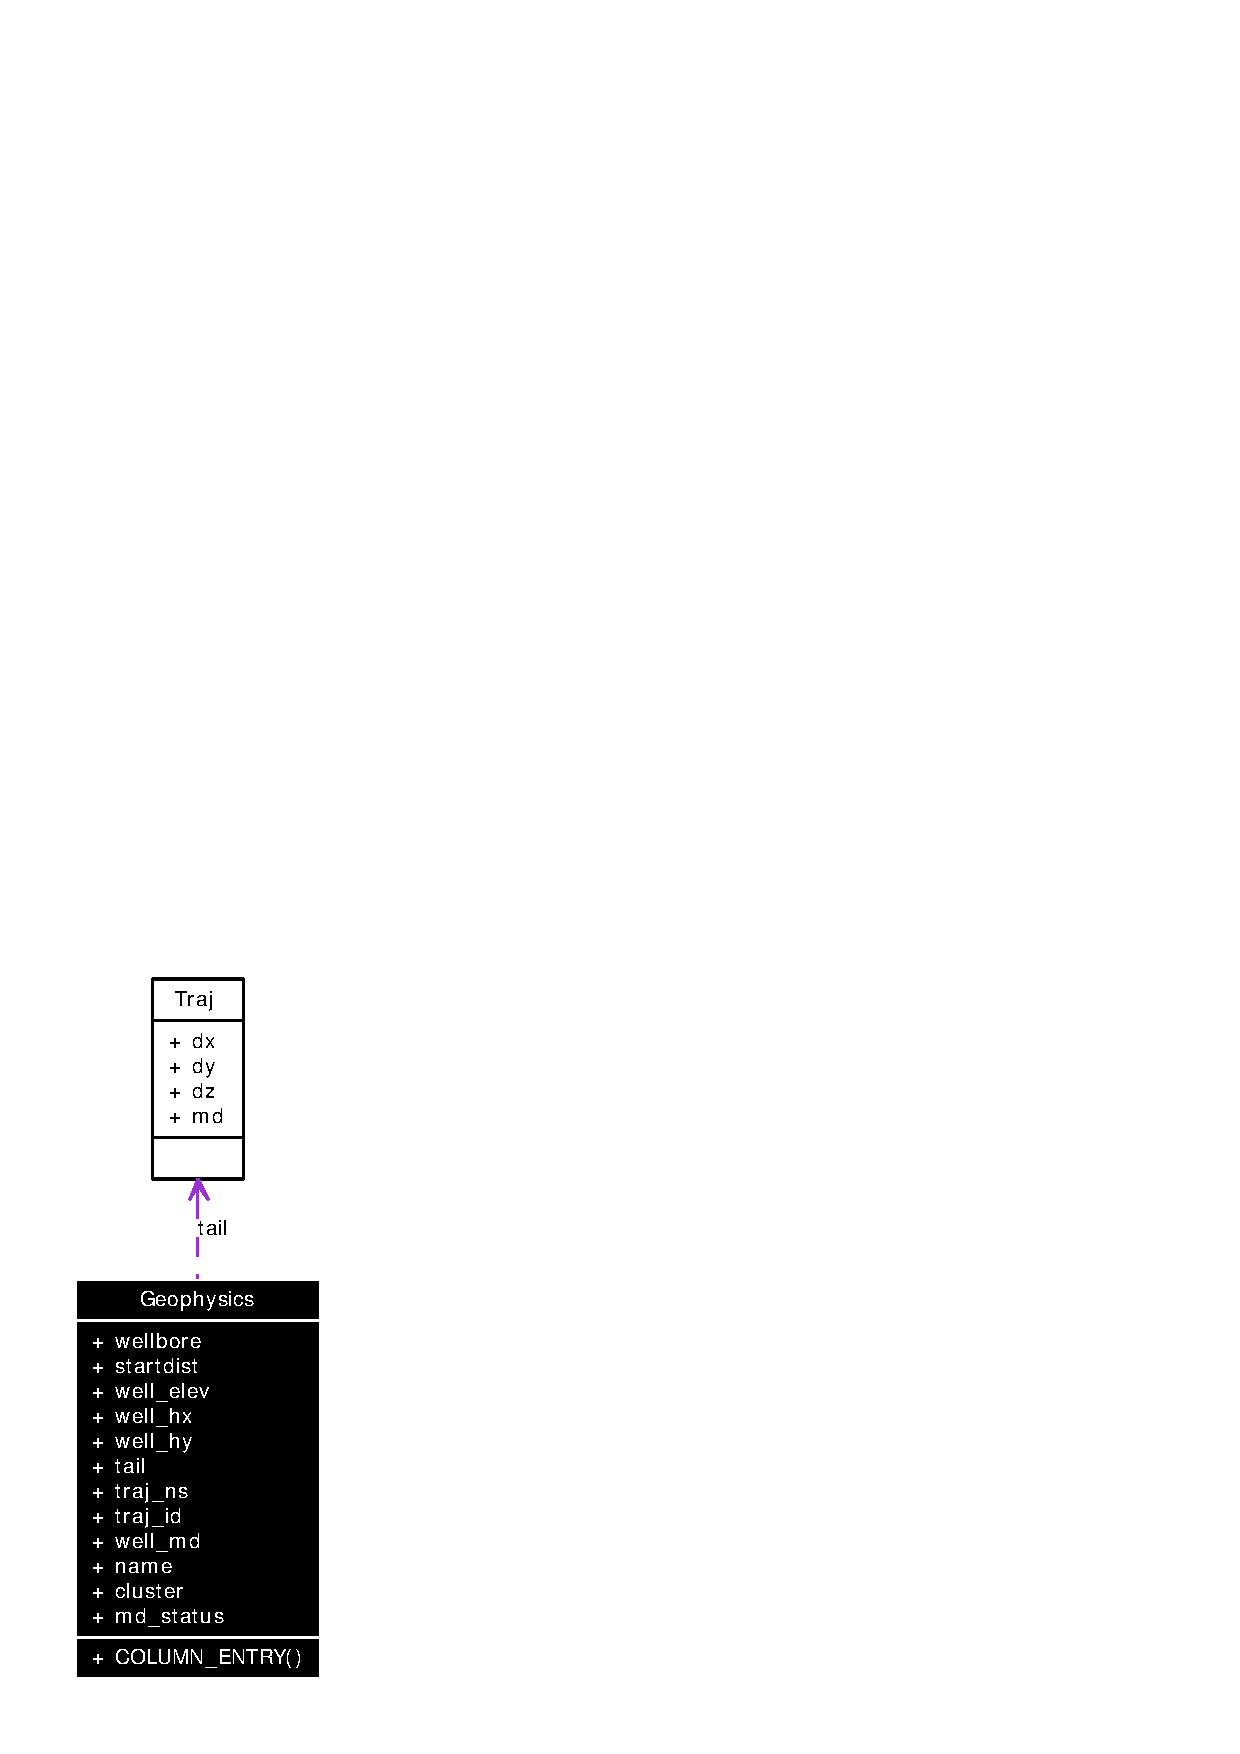
\includegraphics[width=77pt]{struct_geophysics__coll__graph}
\end{center}
\end{figure}
\subsection*{Public Member Functions}
\begin{CompactItemize}
\item 
{\bf COLUMN\_\-ENTRY} (13, {\bf name})\label{struct_geophysics_a0}

\end{CompactItemize}
\subsection*{Public Attributes}
\begin{CompactItemize}
\item 
long {\bf wellbore}\label{struct_geophysics_o0}

\item 
float {\bf startdist}\label{struct_geophysics_o1}

\item 
float {\bf well\_\-elev}\label{struct_geophysics_o2}

\item 
float {\bf well\_\-hx}\label{struct_geophysics_o3}

\item 
float {\bf well\_\-hy}\label{struct_geophysics_o4}

\item 
{\bf Traj} {\bf tail}\label{struct_geophysics_o5}

\item 
short {\bf traj\_\-ns}\label{struct_geophysics_o6}

\item 
unsigned char {\bf traj\_\-id}\label{struct_geophysics_o7}

\item 
float {\bf well\_\-md}\label{struct_geophysics_o8}

\item 
char {\bf name} [32]\label{struct_geophysics_o9}

\item 
long {\bf cluster}\label{struct_geophysics_o10}

\item 
DBSTATUS {\bf md\_\-status}\label{struct_geophysics_o11}

\end{CompactItemize}


\subsection{Detailed Description}




Definition at line 31 of file surface\_\-pick.cpp.

The documentation for this struct was generated from the following file:\begin{CompactItemize}
\item 
surface\_\-pick.cpp\end{CompactItemize}

\section{glyph\_\-type Struct Reference}
\label{structglyph__type}\index{glyph_type@{glyph\_\-type}}
\subsection*{Public Attributes}
\begin{CompactItemize}
\item 
char {\bf ch} [2]\label{structglyph__type_o0}

\item 
double {\bf ww}\label{structglyph__type_o1}

\item 
double {\bf x1}\label{structglyph__type_o2}

\item 
double {\bf y1}\label{structglyph__type_o3}

\item 
double {\bf x2}\label{structglyph__type_o4}

\item 
double {\bf y2}\label{structglyph__type_o5}

\item 
double {\bf nx}\label{structglyph__type_o6}

\item 
double {\bf ny}\label{structglyph__type_o7}

\item 
double {\bf x0}\label{structglyph__type_o8}

\item 
double {\bf y0}\label{structglyph__type_o9}

\item 
double {\bf a}\label{structglyph__type_o10}

\end{CompactItemize}


\subsection{Detailed Description}




Definition at line 385 of file ps\_\-text.cpp.

The documentation for this struct was generated from the following file:\begin{CompactItemize}
\item 
ps\_\-text.cpp\end{CompactItemize}

\section{grid\_\-type Struct Reference}
\label{structgrid__type}\index{grid_type@{grid\_\-type}}
\subsection*{Public Attributes}
\begin{CompactItemize}
\item 
short {\bf cx}\label{structgrid__type_o0}

\item 
short {\bf cy}\label{structgrid__type_o1}

\item 
double {\bf x1}\label{structgrid__type_o2}

\item 
double {\bf x2}\label{structgrid__type_o3}

\item 
double {\bf y1}\label{structgrid__type_o4}

\item 
double {\bf y2}\label{structgrid__type_o5}

\item 
double {\bf z1}\label{structgrid__type_o6}

\item 
double {\bf z2}\label{structgrid__type_o7}

\item 
float $\ast$ {\bf zz}\label{structgrid__type_o8}

\end{CompactItemize}


\subsection{Detailed Description}




Definition at line 60 of file ps\_\-data.h.

The documentation for this struct was generated from the following file:\begin{CompactItemize}
\item 
ps\_\-data.h\end{CompactItemize}

\section{gs\_\-lexord Class Reference}
\label{classgs__lexord}\index{gs_lexord@{gs\_\-lexord}}
Collaboration diagram for gs\_\-lexord:\begin{figure}[H]
\begin{center}
\leavevmode
\includegraphics[width=62pt]{classgs__lexord__coll__graph}
\end{center}
\end{figure}
\subsection*{Public Member Functions}
\begin{CompactItemize}
\item 
{\bf gs\_\-lexord} (const {\bf coord\_\-type} $\ast$v)\label{classgs__lexord_a0}

\item 
bool {\bf operator()} (int n1, int n2) const \label{classgs__lexord_a1}

\end{CompactItemize}


\subsection{Detailed Description}




Definition at line 293 of file ps\_\-cross.cpp.

The documentation for this class was generated from the following file:\begin{CompactItemize}
\item 
ps\_\-cross.cpp\end{CompactItemize}

\section{gs\_\-polord Class Reference}
\label{classgs__polord}\index{gs_polord@{gs\_\-polord}}
Collaboration diagram for gs\_\-polord:\begin{figure}[H]
\begin{center}
\leavevmode
\includegraphics[width=62pt]{classgs__polord__coll__graph}
\end{center}
\end{figure}
\subsection*{Public Member Functions}
\begin{CompactItemize}
\item 
{\bf gs\_\-polord} (const {\bf coord\_\-type} $\ast$v, const {\bf coord\_\-type} $\ast$o)\label{classgs__polord_a0}

\item 
bool {\bf operator()} (int n1, int n2) const \label{classgs__polord_a1}

\end{CompactItemize}


\subsection{Detailed Description}




Definition at line 307 of file ps\_\-cross.cpp.

The documentation for this class was generated from the following file:\begin{CompactItemize}
\item 
ps\_\-cross.cpp\end{CompactItemize}

\section{half\_\-space Class Reference}
\label{classhalf__space}\index{half_space@{half\_\-space}}
Inheritance diagram for half\_\-space:\begin{figure}[H]
\begin{center}
\leavevmode
\includegraphics[width=63pt]{classhalf__space__inherit__graph}
\end{center}
\end{figure}
Collaboration diagram for half\_\-space:\begin{figure}[H]
\begin{center}
\leavevmode
\includegraphics[width=63pt]{classhalf__space__coll__graph}
\end{center}
\end{figure}
\subsection*{Public Member Functions}
\begin{CompactItemize}
\item 
{\bf half\_\-space} (const well\_\-graph \&g, double x1, double y1, double x2, double y2)\label{classhalf__space_a0}

\item 
double {\bf apply} (leda\_\-node n) const \label{classhalf__space_a1}

\end{CompactItemize}


\subsection{Detailed Description}




Definition at line 338 of file wellgrid.cpp.

The documentation for this class was generated from the following file:\begin{CompactItemize}
\item 
wellgrid.cpp\end{CompactItemize}

\section{hull\_\-type Struct Reference}
\label{structhull__type}\index{hull_type@{hull\_\-type}}
\subsection*{Public Attributes}
\begin{CompactItemize}
\item 
int {\bf level}\label{structhull__type_o0}

\item 
int {\bf point}\label{structhull__type_o1}

\item 
double {\bf distance}\label{structhull__type_o2}

\end{CompactItemize}


\subsection{Detailed Description}




Definition at line 73 of file ps\_\-conrec.cpp.

The documentation for this struct was generated from the following file:\begin{CompactItemize}
\item 
ps\_\-conrec.cpp\end{CompactItemize}

\section{label\_\-site Struct Reference}
\label{structlabel__site}\index{label_site@{label\_\-site}}
Collaboration diagram for label\_\-site:\begin{figure}[H]
\begin{center}
\leavevmode
\includegraphics[width=65pt]{structlabel__site__coll__graph}
\end{center}
\end{figure}
\subsection*{Public Attributes}
\begin{CompactItemize}
\item 
char {\bf text} [16]\label{structlabel__site_o0}

\item 
double {\bf xcoord}\label{structlabel__site_o1}

\item 
double {\bf ycoord}\label{structlabel__site_o2}

\item 
double {\bf bbox} [4]\label{structlabel__site_o3}

\item 
double {\bf state} [4]\label{structlabel__site_o4}

\item 
double {\bf param}\label{structlabel__site_o5}

\item 
double {\bf radius}\label{structlabel__site_o6}

\item 
int {\bf cost}\label{structlabel__site_o7}

\item 
int {\bf degree}\label{structlabel__site_o8}

\item 
{\bf label\_\-site} $\ast$$\ast$ {\bf cfl}\label{structlabel__site_o9}

\end{CompactItemize}


\subsection{Detailed Description}




Definition at line 77 of file ps\_\-data.h.

The documentation for this struct was generated from the following file:\begin{CompactItemize}
\item 
ps\_\-data.h\end{CompactItemize}

\section{Label\-Problem Struct Reference}
\label{struct_label_problem}\index{LabelProblem@{LabelProblem}}
Collaboration diagram for Label\-Problem:\begin{figure}[H]
\begin{center}
\leavevmode
\includegraphics[width=70pt]{struct_label_problem__coll__graph}
\end{center}
\end{figure}
\subsection*{Public Attributes}
\begin{CompactItemize}
\item 
int {\bf num\-Sites}\label{struct_label_problem_o0}

\item 
{\bf Label\-Site} $\ast$$\ast$ {\bf site}\label{struct_label_problem_o1}

\end{CompactItemize}


\subsection{Detailed Description}




Definition at line 101 of file ps\_\-label.0.cpp.

The documentation for this struct was generated from the following file:\begin{CompactItemize}
\item 
ps\_\-label.0.cpp\end{CompactItemize}

\section{Label\-Site Struct Reference}
\label{struct_label_site}\index{LabelSite@{LabelSite}}
Collaboration diagram for Label\-Site:\begin{figure}[H]
\begin{center}
\leavevmode
\includegraphics[width=64pt]{struct_label_site__coll__graph}
\end{center}
\end{figure}
\subsection*{Public Attributes}
\begin{CompactItemize}
\item 
char {\bf text} [16]\label{struct_label_site_o0}

\item 
double {\bf xcoord}\label{struct_label_site_o1}

\item 
double {\bf ycoord}\label{struct_label_site_o2}

\item 
double {\bf bbox} [4]\label{struct_label_site_o3}

\item 
double {\bf state} [4]\label{struct_label_site_o4}

\item 
double {\bf param}\label{struct_label_site_o5}

\item 
double {\bf radius}\label{struct_label_site_o6}

\item 
int {\bf cost}\label{struct_label_site_o7}

\item 
int {\bf degree}\label{struct_label_site_o8}

\item 
{\bf Label\-Site} $\ast$$\ast$ {\bf cfl}\label{struct_label_site_o9}

\end{CompactItemize}


\subsection{Detailed Description}




Definition at line 87 of file ps\_\-label.0.cpp.

The documentation for this struct was generated from the following file:\begin{CompactItemize}
\item 
ps\_\-label.0.cpp\end{CompactItemize}

\section{lexord\_\-cmp Class Reference}
\label{classlexord__cmp}\index{lexord_cmp@{lexord\_\-cmp}}
Collaboration diagram for lexord\_\-cmp:\begin{figure}[H]
\begin{center}
\leavevmode
\includegraphics[width=65pt]{classlexord__cmp__coll__graph}
\end{center}
\end{figure}
\subsection*{Public Member Functions}
\begin{CompactItemize}
\item 
{\bf lexord\_\-cmp} (const {\bf coord\_\-type} $\ast$v)\label{classlexord__cmp_a0}

\item 
bool {\bf operator()} (int n1, int n2) const \label{classlexord__cmp_a1}

\end{CompactItemize}


\subsection{Detailed Description}




Definition at line 617 of file ps\_\-cross.cpp.

The documentation for this class was generated from the following file:\begin{CompactItemize}
\item 
ps\_\-cross.cpp\end{CompactItemize}

\section{noddle\_\-type Struct Reference}
\label{structnoddle__type}\index{noddle_type@{noddle\_\-type}}
Collaboration diagram for noddle\_\-type:\begin{figure}[H]
\begin{center}
\leavevmode
\includegraphics[width=57pt]{structnoddle__type__coll__graph}
\end{center}
\end{figure}
\subsection*{Public Attributes}
\begin{CompactItemize}
\item 
{\bf coord\_\-type} {\bf center}\label{structnoddle__type_o0}

\item 
double {\bf angle}\label{structnoddle__type_o1}

\end{CompactItemize}


\subsection{Detailed Description}




Definition at line 69 of file ps\_\-data.h.

The documentation for this struct was generated from the following file:\begin{CompactItemize}
\item 
ps\_\-data.h\end{CompactItemize}

\section{Node Union Reference}
\label{union_node}\index{Node@{Node}}
Collaboration diagram for Node:\begin{figure}[H]
\begin{center}
\leavevmode
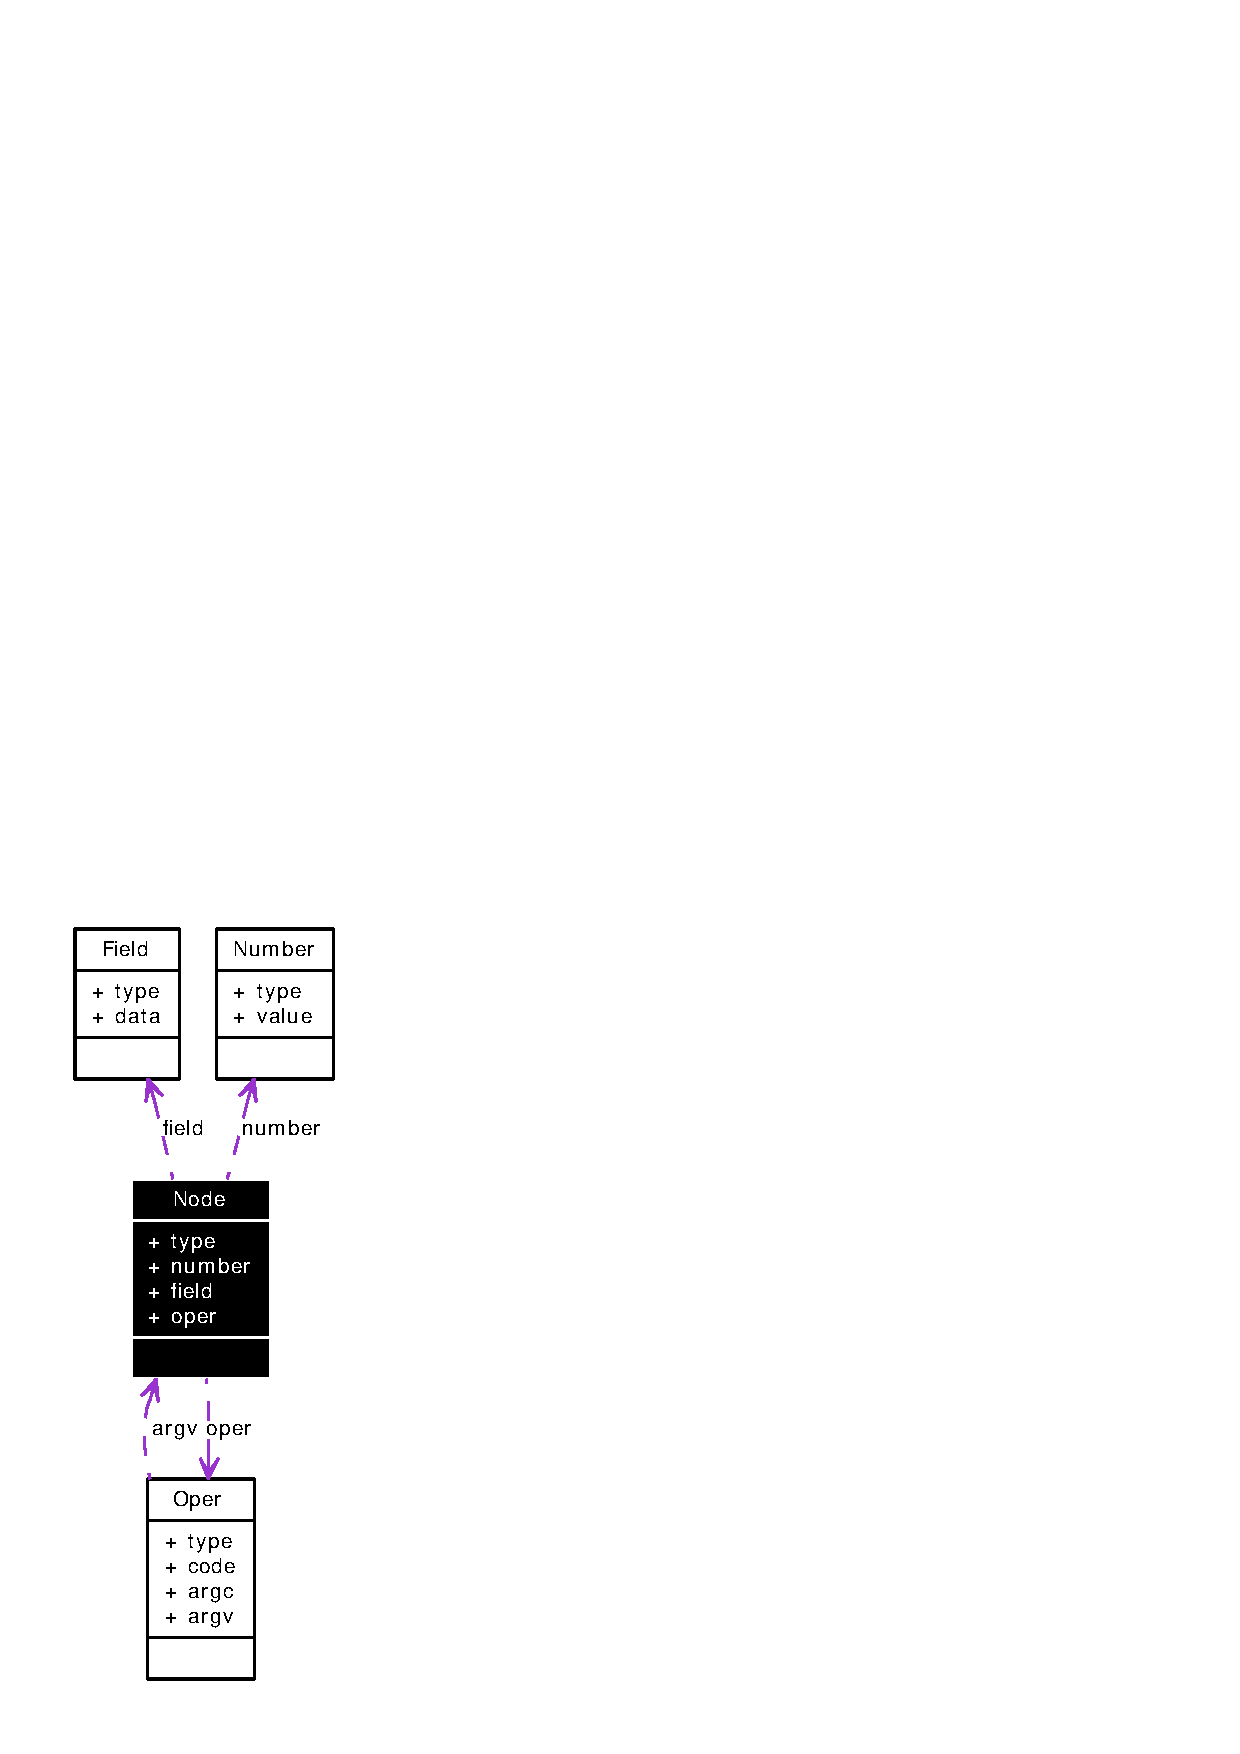
\includegraphics[width=86pt]{union_node__coll__graph}
\end{center}
\end{figure}
\subsection*{Public Attributes}
\begin{CompactItemize}
\item 
Type {\bf type}\label{union_node_o0}

\item 
{\bf Number} {\bf number}\label{union_node_o1}

\item 
{\bf Field} {\bf field}\label{union_node_o2}

\item 
{\bf Oper} {\bf oper}\label{union_node_o3}

\end{CompactItemize}


\subsection{Detailed Description}




Definition at line 120 of file calc.tab.cpp.

The documentation for this union was generated from the following file:\begin{CompactItemize}
\item 
calc.tab.cpp\end{CompactItemize}

\section{node\_\-func Class Reference}
\label{classnode__func}\index{node_func@{node\_\-func}}
Inheritance diagram for node\_\-func:\begin{figure}[H]
\begin{center}
\leavevmode
\includegraphics[width=63pt]{classnode__func__inherit__graph}
\end{center}
\end{figure}
\subsection*{Public Member Functions}
\begin{CompactItemize}
\item 
{\bf node\_\-func} (const well\_\-graph \&init)\label{classnode__func_a0}

\item 
virtual double {\bf apply} (leda\_\-node n) const =0\label{classnode__func_a1}

\item 
const well\_\-graph \& {\bf dom} () const \label{classnode__func_a2}

\end{CompactItemize}


\subsection{Detailed Description}




Definition at line 327 of file wellgrid.cpp.

The documentation for this class was generated from the following file:\begin{CompactItemize}
\item 
wellgrid.cpp\end{CompactItemize}

\section{Number Struct Reference}
\label{struct_number}\index{Number@{Number}}
\subsection*{Public Attributes}
\begin{CompactItemize}
\item 
Type {\bf type}\label{struct_number_o0}

\item 
float {\bf value}\label{struct_number_o1}

\end{CompactItemize}


\subsection{Detailed Description}




Definition at line 100 of file calc.tab.cpp.

The documentation for this struct was generated from the following file:\begin{CompactItemize}
\item 
calc.tab.cpp\end{CompactItemize}

\section{Oper Struct Reference}
\label{struct_oper}\index{Oper@{Oper}}
Collaboration diagram for Oper:\begin{figure}[H]
\begin{center}
\leavevmode
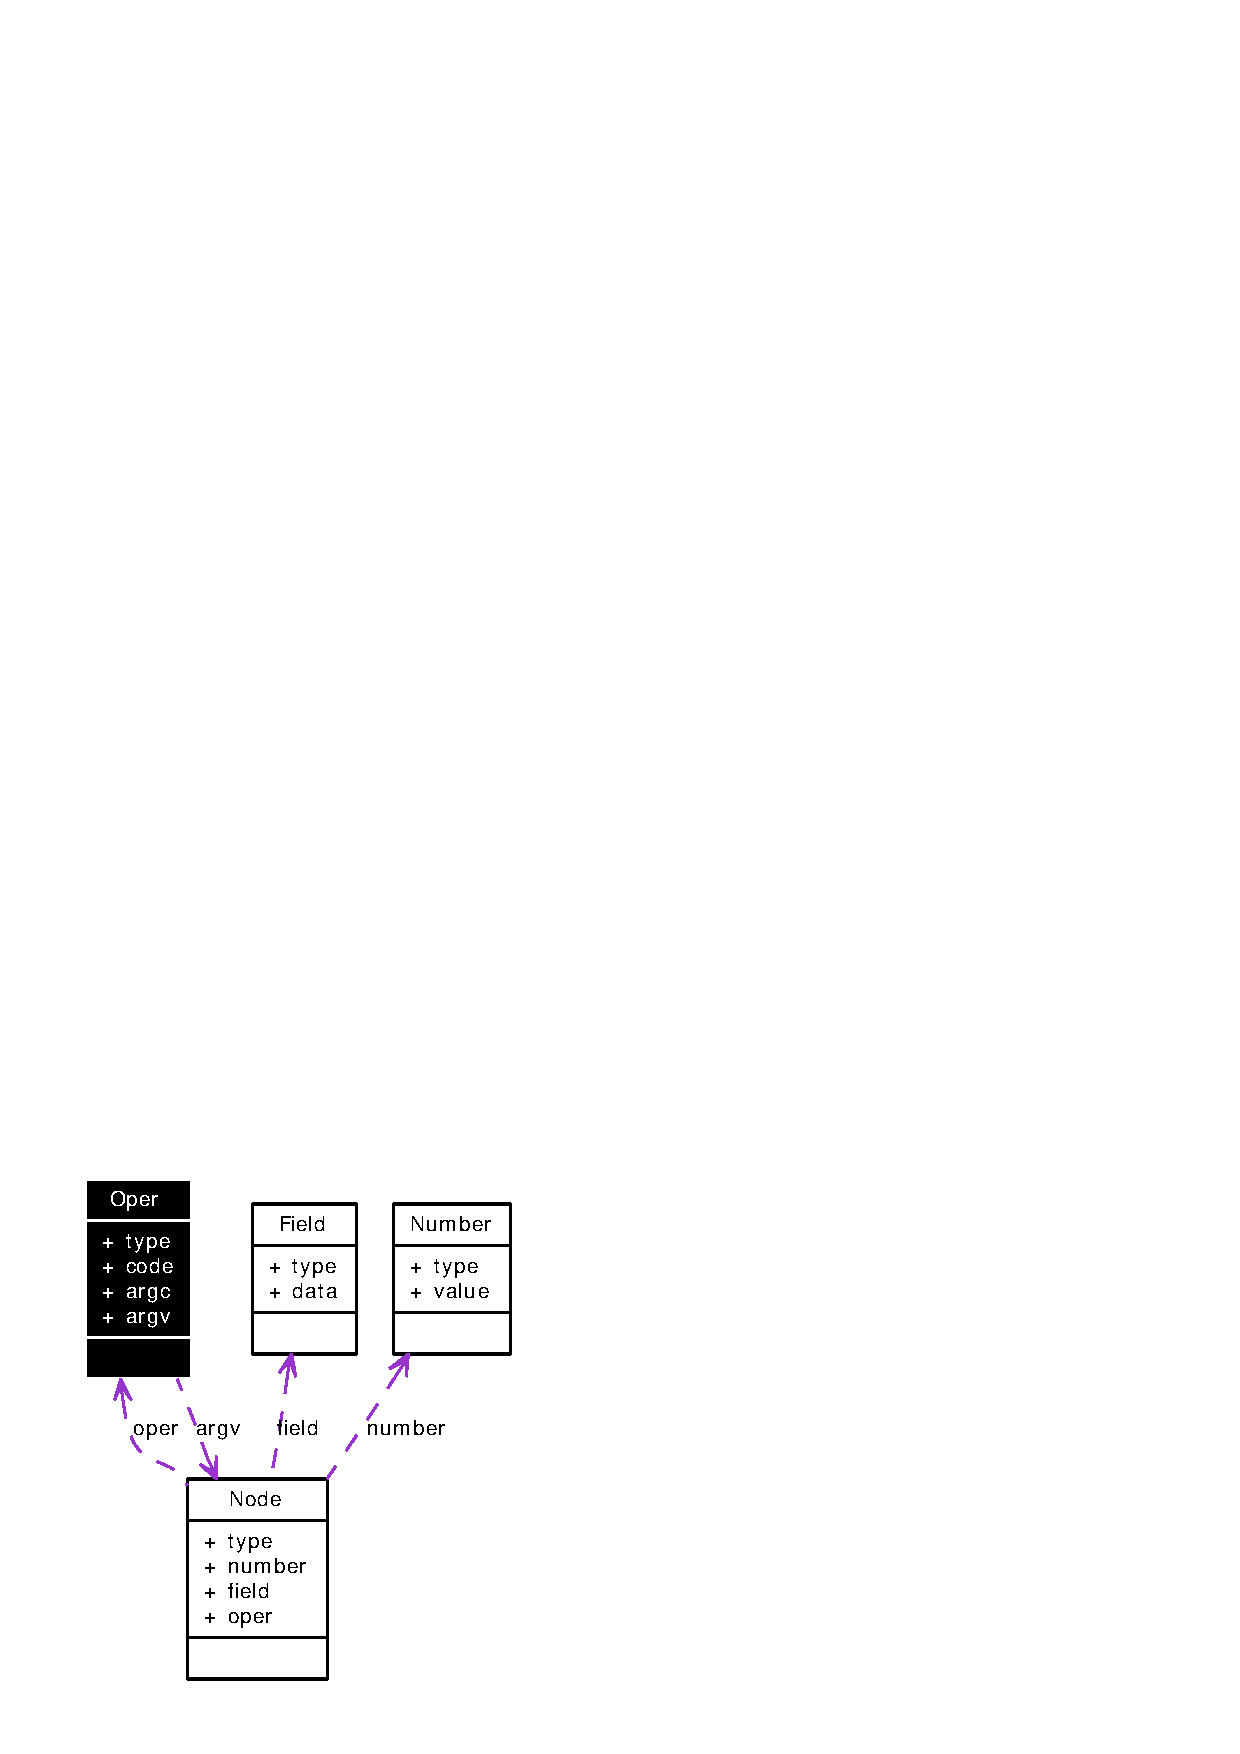
\includegraphics[width=128pt]{struct_oper__coll__graph}
\end{center}
\end{figure}
\subsection*{Public Attributes}
\begin{CompactItemize}
\item 
Type {\bf type}\label{struct_oper_o0}

\item 
Code {\bf code}\label{struct_oper_o1}

\item 
int {\bf argc}\label{struct_oper_o2}

\item 
{\bf Node} $\ast$ {\bf argv} [1]\label{struct_oper_o3}

\end{CompactItemize}


\subsection{Detailed Description}




Definition at line 112 of file calc.tab.cpp.

The documentation for this struct was generated from the following file:\begin{CompactItemize}
\item 
calc.tab.cpp\end{CompactItemize}

\section{pgn\_\-builder Struct Reference}
\label{structpgn__builder}\index{pgn_builder@{pgn\_\-builder}}
Inheritance diagram for pgn\_\-builder:\begin{figure}[H]
\begin{center}
\leavevmode
\includegraphics[width=128pt]{structpgn__builder__inherit__graph}
\end{center}
\end{figure}
\subsection*{Public Member Functions}
\begin{CompactItemize}
\item 
virtual int {\bf new\_\-vertex} (double x, double y)=0\label{structpgn__builder_a0}

\item 
virtual void {\bf begin\_\-curve} ()=0\label{structpgn__builder_a1}

\item 
virtual void {\bf add\_\-vertex} (int)=0\label{structpgn__builder_a2}

\item 
virtual void {\bf end\_\-curve} ()=0\label{structpgn__builder_a3}

\end{CompactItemize}


\subsection{Detailed Description}




Definition at line 219 of file ps\_\-data.h.

The documentation for this struct was generated from the following file:\begin{CompactItemize}
\item 
ps\_\-data.h\end{CompactItemize}

\section{polygon\_\-grid Class Reference}
\label{classpolygon__grid}\index{polygon_grid@{polygon\_\-grid}}
\subsection*{Public Member Functions}
\begin{CompactItemize}
\item 
double {\bf left} (int i) const \label{classpolygon__grid_a0}

\item 
double {\bf right} (int i) const \label{classpolygon__grid_a1}

\item 
double {\bf top} (int j) const \label{classpolygon__grid_a2}

\item 
double {\bf bottom} (int j) const \label{classpolygon__grid_a3}

\item 
double {\bf inf} (int i, int j) const \label{classpolygon__grid_a4}

\item 
void {\bf populate} (int n, double x[$\,$], double y[$\,$])\label{classpolygon__grid_a5}

\item 
{\bf polygon\_\-grid} (int cx, int cy, double x1, double x2, double y1, double y2)\label{classpolygon__grid_a6}

\item 
{\bf polygon\_\-grid} (int cx, int cy, double $\ast$init\_\-x, double $\ast$init\_\-y)\label{classpolygon__grid_a7}

\item 
{\bf $\sim$polygon\_\-grid} ()\label{classpolygon__grid_a8}

\end{CompactItemize}


\subsection{Detailed Description}




Definition at line 1116 of file wellgrid.cpp.

The documentation for this class was generated from the following file:\begin{CompactItemize}
\item 
wellgrid.cpp\end{CompactItemize}

\section{psstream Class Reference}
\label{classpsstream}\index{psstream@{psstream}}
Collaboration diagram for psstream:\begin{figure}[H]
\begin{center}
\leavevmode
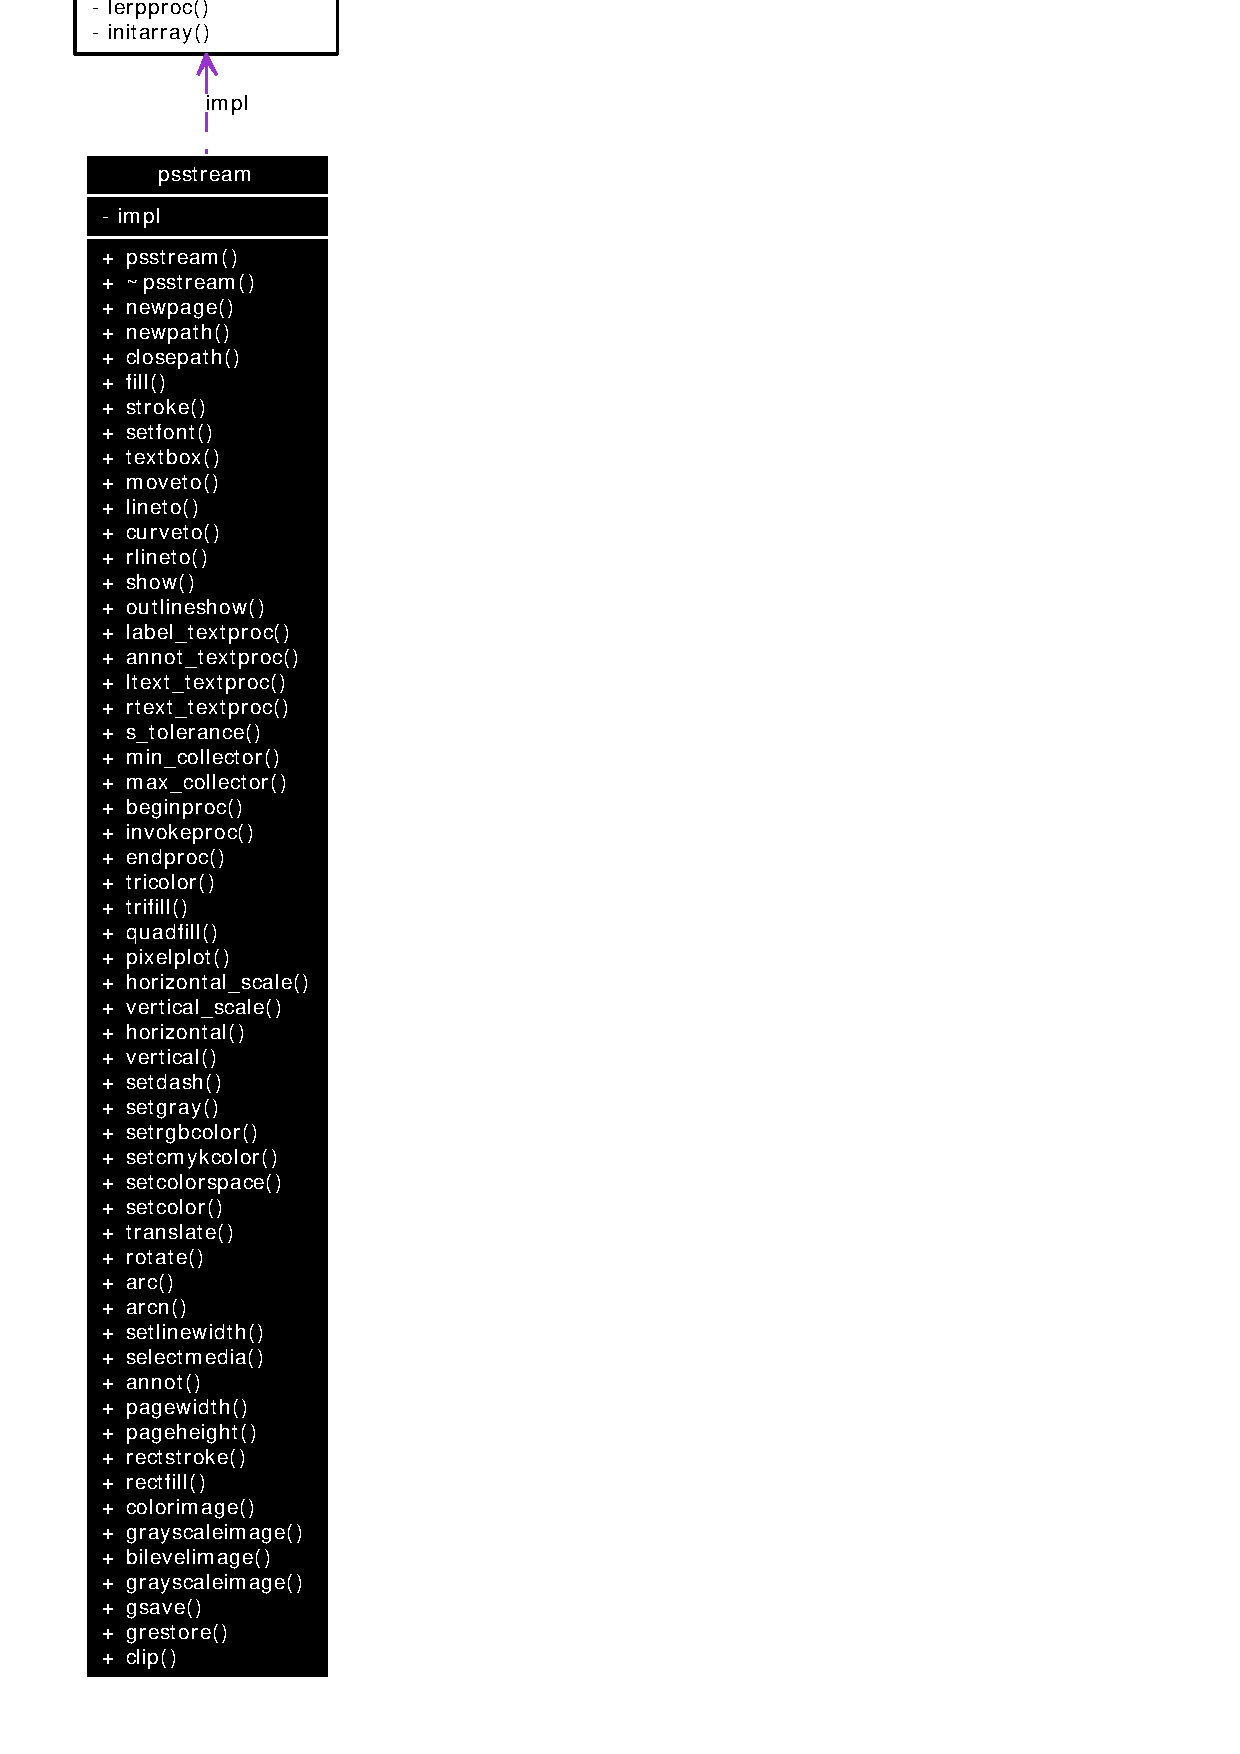
\includegraphics[width=81pt]{classpsstream__coll__graph}
\end{center}
\end{figure}
\subsection*{Public Types}
\begin{CompactItemize}
\item 
enum {\bf Orientation} \{ {\bf PORTRAIT}, 
{\bf LANDSCAPE}
 \}
\item 
enum {\bf Format} \{ {\bf FORMAT\_\-A4}, 
{\bf FORMAT\_\-A3}, 
{\bf FORMAT\_\-A0}, 
{\bf FORMAT\_\-NUM}
 \}
\item 
enum {\bf Pattern} \{ \par
{\bf BDIAGONAL}, 
{\bf CROSSHATCH}, 
{\bf DIAGHATCH}, 
{\bf HORIZONTAL}, 
\par
{\bf FDIAGONAL}, 
{\bf VERTICAL}, 
{\bf SANDSTONE}, 
{\bf SHALE}, 
\par
{\bf LIMESTONE}, 
{\bf DOLOMITE}, 
{\bf SILICATE}, 
{\bf SALT}, 
\par
{\bf ANHYDRITE}, 
{\bf SILTSTONE}, 
{\bf BITUMEN}, 
{\bf OILZONE}, 
\par
{\bf WATZONE}, 
{\bf GASZONE}, 
{\bf GYPSUM}, 
{\bf DEEPBASE}, 
\par
{\bf GASOILZONE}, 
{\bf OILWATZONE}, 
{\bf GASWATZONE}, 
{\bf GASOILWATZONE}, 
\par
{\bf WATGASZONE}, 
{\bf WATOILZONE}, 
{\bf OILGASZONE}, 
{\bf SAND}, 
\par
{\bf COAL}, 
{\bf EVALUATION}, 
{\bf NUM\_\-PATTERNS}
 \}
\item 
enum {\bf Annot} \{ {\bf ANNOT\_\-LEFT}, 
{\bf ANNOT\_\-CENTER}, 
{\bf ANNOT\_\-RIGHT}
 \}
\item 
enum {\bf Justify} \{ \par
{\bf LABEL\_\-E}, 
{\bf LABEL\_\-N}, 
{\bf LABEL\_\-W}, 
{\bf LABEL\_\-S}, 
\par
{\bf LABEL\_\-NE}, 
{\bf LABEL\_\-NW}, 
{\bf LABEL\_\-SE}, 
{\bf LABEL\_\-SW}, 
\par
{\bf LABEL\_\-NONE}
 \}
\end{CompactItemize}
\subsection*{Public Member Functions}
\begin{CompactItemize}
\item 
{\bf psstream} (const char $\ast$file)\label{classpsstream_a0}

\item 
{\bf $\sim$psstream} ()\label{classpsstream_a1}

\item 
void {\bf newpage} ()\label{classpsstream_a2}

\item 
void {\bf newpath} ()\label{classpsstream_a3}

\item 
void {\bf closepath} ()\label{classpsstream_a4}

\item 
void {\bf fill} ()\label{classpsstream_a5}

\item 
void {\bf stroke} ()\label{classpsstream_a6}

\item 
bool {\bf setfont} (const char $\ast$name, double size)\label{classpsstream_a7}

\item 
void {\bf textbox} (const char $\ast$text, double $\ast${\bf bbox})\label{classpsstream_a8}

\item 
void {\bf moveto} (double x, double y)\label{classpsstream_a9}

\item 
void {\bf lineto} (double x, double y)\label{classpsstream_a10}

\item 
void {\bf curveto} (double x1, double y1, double x2, double y2, double x3, double y3)\label{classpsstream_a11}

\item 
void {\bf rlineto} (double x, double y)\label{classpsstream_a12}

\item 
void {\bf show} (const char $\ast$text)\label{classpsstream_a13}

\item 
void {\bf outlineshow} (const char $\ast$text)\label{classpsstream_a14}

\item 
void {\bf label\_\-textproc} (double x, double y, double r, double d, const char $\ast$s, bool f)\label{classpsstream_a15}

\item 
void {\bf annot\_\-textproc} (double x, double y, double a, const char $\ast$s, bool f)\label{classpsstream_a16}

\item 
void {\bf ltext\_\-textproc} (double x, double y, double r, double a, const char $\ast$s, bool f)\label{classpsstream_a17}

\item 
void {\bf rtext\_\-textproc} (double x, double y, double r, double a, const char $\ast$s, bool f)\label{classpsstream_a18}

\item 
void {\bf s\_\-tolerance} (double s)\label{classpsstream_a19}

\item 
void {\bf min\_\-collector} (double p, double r, double g, double b)\label{classpsstream_a20}

\item 
void {\bf max\_\-collector} (double p, double r, double g, double b)\label{classpsstream_a21}

\item 
void {\bf beginproc} (const char $\ast$name)\label{classpsstream_a22}

\item 
void {\bf invokeproc} (const char $\ast$name)\label{classpsstream_a23}

\item 
void {\bf endproc} ()\label{classpsstream_a24}

\item 
void {\bf tricolor} (int n, const {\bf color\_\-type} $\ast$s)\label{classpsstream_a25}

\item 
void {\bf trifill} (double x1, double y1, double g1, double o1, double w1, double x2, double y2, double g2, double o2, double w2, double x3, double y3, double g3, double o3, double w3)\label{classpsstream_a26}

\item 
void {\bf quadfill} (double x1, double y1, double g1, double o1, double w1, double x2, double y2, double g2, double o2, double w2, double x3, double y3, double g3, double o3, double w3, double x4, double y4, double g4, double o4, double w4)\label{classpsstream_a27}

\item 
void {\bf pixelplot} (int cx, int cy, const float $\ast$xx, const float $\ast$yy, const float $\ast$gg, const float $\ast$oo, const float $\ast$ww)\label{classpsstream_a28}

\item 
void {\bf horizontal\_\-scale} (int start, int step, int final, double orig, double range, double dx, double x0, double y0, double sy)\label{classpsstream_a29}

\item 
void {\bf vertical\_\-scale} (int start, int step, int final, double orig, double range, double dy, double x0, double y0, double sx)\label{classpsstream_a30}

\item 
void {\bf horizontal} (const {\bf Scale} \&scale)\label{classpsstream_a31}

\item 
void {\bf vertical} (const {\bf Scale} \&scale)\label{classpsstream_a32}

\item 
void {\bf setdash} (int n, int $\ast$pp, int o)\label{classpsstream_a33}

\item 
void {\bf setgray} (double g)\label{classpsstream_a34}

\item 
void {\bf setrgbcolor} (double r, double g, double b)\label{classpsstream_a35}

\item 
void {\bf setcmykcolor} (double c, double m, double y, double k)\label{classpsstream_a36}

\item 
void {\bf setcolorspace} (double line\_\-width, double scale\_\-factor)\label{classpsstream_a37}

\item 
void {\bf setcolor} (double r, double g, double b, {\bf Pattern} h)\label{classpsstream_a38}

\item 
void {\bf translate} (double x, double y)\label{classpsstream_a39}

\item 
void {\bf rotate} (double a)\label{classpsstream_a40}

\item 
void {\bf arc} (double x, double y, double r, double a1, double a2)\label{classpsstream_a41}

\item 
void {\bf arcn} (double x, double y, double r, double a1, double a2)\label{classpsstream_a42}

\item 
void {\bf setlinewidth} (double w)\label{classpsstream_a43}

\item 
void {\bf selectmedia} ({\bf Format} f, {\bf Orientation} o)\label{classpsstream_a44}

\item 
void {\bf annot} (double x, double y, double r, double angle,$\backslash${\bf Annot} anchor, bool show, const char $\ast$text, double {\bf bbox}[8])\label{classpsstream_a45}

\item 
double {\bf pagewidth} () const \label{classpsstream_a46}

\item 
double {\bf pageheight} () const \label{classpsstream_a47}

\item 
void {\bf rectstroke} (double x, double y, double w, double h)\label{classpsstream_a48}

\item 
void {\bf rectfill} (double x, double y, double w, double h)\label{classpsstream_a49}

\item 
void {\bf colorimage} (double x0, double y0, double sx, double sy,$\backslash$int num\_\-levels, const float $\ast$level, const {\bf color\_\-type} $\ast$color,$\backslash$int cx, int cy, const float $\ast$func)\label{classpsstream_a50}

\item 
void {\bf grayscaleimage} (double x0, double y0, double sx, double sy,$\backslash$int num\_\-levels, const float $\ast$level, const double $\ast$color,$\backslash$int cx, int cy, const float $\ast$func)\label{classpsstream_a51}

\item 
void {\bf bilevelimage} (double x0, double y0, double sx, double sy,$\backslash$int cx, int cy, const vertex\_\-type \&ver, const edge\_\-type \&pgn)\label{classpsstream_a52}

\item 
void {\bf grayscaleimage} (double x0, double y0, double sx, double sy,$\backslash$int cx, int cy, const vertex\_\-type \&ver, const edge\_\-type \&pgn)\label{classpsstream_a53}

\item 
void {\bf gsave} ()\label{classpsstream_a54}

\item 
void {\bf grestore} ()\label{classpsstream_a55}

\item 
void {\bf clip} ()\label{classpsstream_a56}

\end{CompactItemize}
\subsection*{Classes}
\begin{CompactItemize}
\item 
struct {\bf Scale}
\end{CompactItemize}


\subsection{Detailed Description}




Definition at line 92 of file ps\_\-data.h.

The documentation for this class was generated from the following files:\begin{CompactItemize}
\item 
ps\_\-data.h\item 
ps\_\-image.cpp\item 
ps\_\-proc.0.cpp\item 
ps\_\-proc.cpp\item 
ps\_\-stream.cpp\end{CompactItemize}

\section{psstream::Scale Struct Reference}
\label{structpsstream_1_1_scale}\index{psstream::Scale@{psstream::Scale}}
Collaboration diagram for psstream::Scale:\begin{figure}[H]
\begin{center}
\leavevmode
\includegraphics[width=67pt]{structpsstream_1_1_scale__coll__graph}
\end{center}
\end{figure}
\subsection*{Public Types}
\begin{CompactItemize}
\item 
enum {\bf Flags} \{ \par
{\bf HAS\_\-INNER\_\-TICK} =  1, 
{\bf HAS\_\-OUTER\_\-TICK} =  2, 
{\bf HAS\_\-AXIS\_\-LINE} =  4, 
{\bf HAS\_\-LABEL\_\-TEXT} =  8, 
\par
{\bf HAS\_\-GRID\_\-LINES} =  16, 
{\bf HAS\_\-INNER\_\-FRAME} =  32, 
{\bf HAS\_\-OUTER\_\-FRAME} =  64, 
{\bf HAS\_\-COLOR\_\-BOX} =  128
 \}
\item 
enum {\bf Type} \{ {\bf ARITHMETIC}, 
{\bf LOGARITHMIC}, 
{\bf PROBABILITY}
 \}
\end{CompactItemize}
\subsection*{Public Attributes}
\begin{CompactItemize}
\item 
{\bf Type} {\bf type}\label{structpsstream_1_1_scale_o0}

\item 
{\bf Justify} {\bf label}\label{structpsstream_1_1_scale_o1}

\item 
int {\bf flags}\label{structpsstream_1_1_scale_o2}

\item 
double {\bf range} [2]\label{structpsstream_1_1_scale_o3}

\item 
double {\bf region} [4]\label{structpsstream_1_1_scale_o4}

\item 
double {\bf margin}\label{structpsstream_1_1_scale_o5}

\item 
double {\bf tick\_\-length}\label{structpsstream_1_1_scale_o6}

\item 
double {\bf line\_\-width}\label{structpsstream_1_1_scale_o7}

\item 
const char $\ast$ {\bf font\_\-name}\label{structpsstream_1_1_scale_o8}

\item 
double {\bf font\_\-size}\label{structpsstream_1_1_scale_o9}

\item 
{\bf color\_\-type} {\bf color}\label{structpsstream_1_1_scale_o10}

\item 
int {\bf factor}\label{structpsstream_1_1_scale_o11}

\item 
const char $\ast$ {\bf annot}\label{structpsstream_1_1_scale_o12}

\item 
const char $\ast$ {\bf format}\label{structpsstream_1_1_scale_o13}

\item 
const char $\ast$ {\bf units}\label{structpsstream_1_1_scale_o14}

\end{CompactItemize}


\subsection{Detailed Description}




Definition at line 106 of file ps\_\-data.h.

The documentation for this struct was generated from the following file:\begin{CompactItemize}
\item 
ps\_\-data.h\end{CompactItemize}

\section{psstream\_\-impl Class Reference}
\label{classpsstream__impl}\index{psstream_impl@{psstream\_\-impl}}
\subsection*{Public Member Functions}
\begin{CompactItemize}
\item 
{\bf psstream\_\-impl} (const char $\ast$file)\label{classpsstream__impl_a0}

\item 
{\bf $\sim$psstream\_\-impl} ()\label{classpsstream__impl_a1}

\item 
bool {\bf setfont} (const char $\ast$name, double size)\label{classpsstream__impl_a2}

\item 
void {\bf textbox} (const char $\ast$text, double $\ast${\bf bbox})\label{classpsstream__impl_a3}

\item 
void {\bf newpage} ()\label{classpsstream__impl_a4}

\item 
void {\bf moveto} (double x, double y)\label{classpsstream__impl_a5}

\item 
void {\bf lineto} (double x, double y)\label{classpsstream__impl_a6}

\item 
void {\bf curveto} (double x1, double y1, double x2, double y2, double x3, double y3)\label{classpsstream__impl_a7}

\item 
void {\bf rlineto} (double x, double y)\label{classpsstream__impl_a8}

\item 
void {\bf show} (const char $\ast$text)\label{classpsstream__impl_a9}

\item 
void {\bf outlineshow} (const char $\ast$text)\label{classpsstream__impl_a10}

\item 
void {\bf label\_\-textproc} (double x, double y, double r, double d, const char $\ast$s, bool f)\label{classpsstream__impl_a11}

\item 
void {\bf annot\_\-textproc} (double x, double y, double a, const char $\ast$s, bool f)\label{classpsstream__impl_a12}

\item 
void {\bf ltext\_\-textproc} (double x, double y, double r, double a, const char $\ast$s, bool f)\label{classpsstream__impl_a13}

\item 
void {\bf rtext\_\-textproc} (double x, double y, double r, double a, const char $\ast$s, bool f)\label{classpsstream__impl_a14}

\item 
void {\bf s\_\-tolerance} (double s)\label{classpsstream__impl_a15}

\item 
void {\bf min\_\-collector} (double p, double r, double g, double b)\label{classpsstream__impl_a16}

\item 
void {\bf max\_\-collector} (double p, double r, double g, double b)\label{classpsstream__impl_a17}

\item 
void {\bf beginproc} (const char $\ast$name)\label{classpsstream__impl_a18}

\item 
void {\bf invokeproc} (const char $\ast$name)\label{classpsstream__impl_a19}

\item 
void {\bf endproc} ()\label{classpsstream__impl_a20}

\item 
void {\bf tricolor} (int n, const {\bf color\_\-type} $\ast$s)\label{classpsstream__impl_a21}

\item 
void {\bf trifill} (double x1, double y1, double g1, double o1, double w1, double x2, double y2, double g2, double o2, double w2, double x3, double y3, double g3, double o3, double w3)\label{classpsstream__impl_a22}

\item 
void {\bf quadfill} (double x1, double y1, double g1, double o1, double w1, double x2, double y2, double g2, double o2, double w2, double x3, double y3, double g3, double o3, double w3, double x4, double y4, double g4, double o4, double w4)\label{classpsstream__impl_a23}

\item 
void {\bf pixelplot} (int cx, int cy, const float $\ast$xx, const float $\ast$yy, const float $\ast$gg, const float $\ast$oo, const float $\ast$ww)\label{classpsstream__impl_a24}

\item 
void {\bf setdash} (int n, int $\ast$pp, int o)\label{classpsstream__impl_a25}

\item 
void {\bf setgray} (double g)\label{classpsstream__impl_a26}

\item 
void {\bf setrgbcolor} (double r, double g, double b)\label{classpsstream__impl_a27}

\item 
void {\bf setcmykcolor} (double c, double m, double y, double k)\label{classpsstream__impl_a28}

\item 
void {\bf setcolorspace} (double line\_\-width, double scale\_\-factor)\label{classpsstream__impl_a29}

\item 
void {\bf setcolor} (double r, double g, double b, {\bf psstream::Pattern} h)\label{classpsstream__impl_a30}

\item 
void {\bf translate} (double x, double y)\label{classpsstream__impl_a31}

\item 
void {\bf rotate} (double a)\label{classpsstream__impl_a32}

\item 
void {\bf command} (const char $\ast$cmd)\label{classpsstream__impl_a33}

\item 
void {\bf arc} (double x, double y, double r, double a1, double a2)\label{classpsstream__impl_a34}

\item 
void {\bf arcn} (double x, double y, double r, double a1, double a2)\label{classpsstream__impl_a35}

\item 
void {\bf setlinewidth} (double w)\label{classpsstream__impl_a36}

\item 
void {\bf updatebb} (double x1, double x2, double y1, double y2)\label{classpsstream__impl_a37}

\item 
void {\bf updatecp} (double x, double y)\label{classpsstream__impl_a38}

\item 
void {\bf selectmedia} ({\bf psstream::Format} f, {\bf psstream::Orientation} o)\label{classpsstream__impl_a39}

\item 
double {\bf pagewidth} () const \label{classpsstream__impl_a40}

\item 
double {\bf pageheight} () const \label{classpsstream__impl_a41}

\item 
void {\bf rectstroke} (double x, double y, double w, double h)\label{classpsstream__impl_a42}

\item 
void {\bf rectfill} (double x, double y, double w, double h)\label{classpsstream__impl_a43}

\item 
void {\bf colorimage} (double x0, double y0, double sx, double sy,$\backslash$int num\_\-levels, const float $\ast$level, const {\bf color\_\-type} $\ast$color,$\backslash$int cx, int cy, const float $\ast$func)\label{classpsstream__impl_a44}

\item 
void {\bf grayscaleimage} (double x0, double y0, double sx, double sy,$\backslash$int num\_\-levels, const float $\ast$level, const double $\ast$color,$\backslash$int cx, int cy, const float $\ast$func)\label{classpsstream__impl_a45}

\item 
void {\bf bilevelimage} (double x0, double y0, double sx, double sy,$\backslash$int cx, int cy, const vertex\_\-type \&ver, const edge\_\-type \&pgn)\label{classpsstream__impl_a46}

\item 
void {\bf grayscaleimage} (double x0, double y0, double sx, double sy,$\backslash$int cx, int cy, const vertex\_\-type \&ver, const edge\_\-type \&pgn)\label{classpsstream__impl_a47}

\item 
bool {\bf getbbox} (double $\ast$bb)\label{classpsstream__impl_a48}

\item 
void {\bf setbbox} (bool f, double $\ast$bb)\label{classpsstream__impl_a49}

\item 
void {\bf horizontal\_\-scale} (int start, int step, int final, double orig, double range, double dx, double x0, double y0, double sx)\label{classpsstream__impl_a50}

\item 
void {\bf vertical\_\-scale} (int start, int step, int final, double orig, double range, double dy, double x0, double y0, double sx)\label{classpsstream__impl_a51}

\end{CompactItemize}
\subsection*{Classes}
\begin{CompactItemize}
\item 
struct {\bf page\_\-type}
\end{CompactItemize}


\subsection{Detailed Description}




Definition at line 5 of file ps\_\-priv.h.

The documentation for this class was generated from the following files:\begin{CompactItemize}
\item 
ps\_\-priv.h\item 
ps\_\-image.cpp\item 
ps\_\-proc.0.cpp\item 
ps\_\-proc.cpp\item 
ps\_\-stream.cpp\end{CompactItemize}

\section{quant Class Reference}
\label{classquant}\index{quant@{quant}}
\subsection*{Public Member Functions}
\begin{CompactItemize}
\item 
{\bf quant} (double dd)\label{classquant_a0}

\item 
{\bf coord\_\-type} {\bf operator()} (const {\bf coord\_\-type} \&q) const \label{classquant_a1}

\end{CompactItemize}


\subsection{Detailed Description}




Definition at line 25 of file z1.cpp.

The documentation for this class was generated from the following file:\begin{CompactItemize}
\item 
z1.cpp\end{CompactItemize}

\section{s\_\-curve Class Reference}
\label{classs__curve}\index{s_curve@{s\_\-curve}}
\subsection*{Public Member Functions}
\begin{CompactItemize}
\item 
{\bf s\_\-curve} (const vertex\_\-type \&ver, const curve\_\-type \&cur)\label{classs__curve_a0}

\item 
{\bf $\sim$s\_\-curve} ()\label{classs__curve_a1}

\item 
double {\bf length} () const \label{classs__curve_a2}

\item 
void {\bf position} (double s, double $\ast$x, double $\ast$y) const \label{classs__curve_a3}

\item 
bool {\bf forward} (double s, double w, double $\ast$g, double $\ast$dg) const \label{classs__curve_a4}

\item 
bool {\bf backward} (double s, double w, double $\ast$g, double $\ast$dg) const \label{classs__curve_a5}

\item 
bool {\bf is\_\-closed} () const \label{classs__curve_a6}

\end{CompactItemize}


\subsection{Detailed Description}




Definition at line 81 of file ps\_\-text.cpp.

The documentation for this class was generated from the following file:\begin{CompactItemize}
\item 
ps\_\-text.cpp\end{CompactItemize}

\section{Sample Struct Reference}
\label{struct_sample}\index{Sample@{Sample}}
\subsection*{Public Attributes}
\begin{CompactItemize}
\item 
float {\bf sparam}\label{struct_sample_o0}

\item 
float {\bf xcoord}\label{struct_sample_o1}

\item 
float {\bf ycoord}\label{struct_sample_o2}

\end{CompactItemize}


\subsection{Detailed Description}




Definition at line 1 of file surface\_\-pick.h.

The documentation for this struct was generated from the following file:\begin{CompactItemize}
\item 
surface\_\-pick.h\end{CompactItemize}

\section{Segment Struct Reference}
\label{struct_segment}\index{Segment@{Segment}}
\subsection*{Public Attributes}
\begin{CompactItemize}
\item 
double {\bf alpha}\label{struct_segment_o0}

\item 
bool {\bf outgoing}\label{struct_segment_o1}

\end{CompactItemize}


\subsection{Detailed Description}




Definition at line 19 of file ps\_\-bbox.cpp.

The documentation for this struct was generated from the following file:\begin{CompactItemize}
\item 
ps\_\-bbox.cpp\end{CompactItemize}

\section{seqgen Class Reference}
\label{classseqgen}\index{seqgen@{seqgen}}
\subsection*{Public Member Functions}
\begin{CompactItemize}
\item 
{\bf seqgen} (int first)\label{classseqgen_a0}

\item 
int {\bf operator()} ()\label{classseqgen_a1}

\end{CompactItemize}


\subsection{Detailed Description}




Definition at line 14 of file z1.cpp.

The documentation for this class was generated from the following file:\begin{CompactItemize}
\item 
z1.cpp\end{CompactItemize}

\section{SH\_\-zero\_\-compare Class Reference}
\label{class_s_h__zero__compare}\index{SH_zero_compare@{SH\_\-zero\_\-compare}}
Collaboration diagram for SH\_\-zero\_\-compare:\begin{figure}[H]
\begin{center}
\leavevmode
\includegraphics[width=85pt]{class_s_h__zero__compare__coll__graph}
\end{center}
\end{figure}
\subsection*{Public Member Functions}
\begin{CompactItemize}
\item 
{\bf SH\_\-zero\_\-compare} (const {\bf coord\_\-type} $\ast$p, {\bf Zero\_\-type} $\ast$z, double a, double b)\label{class_s_h__zero__compare_a0}

\item 
const {\bf coord\_\-type} $\ast$ {\bf zero} (const {\bf Zero\_\-type} $\ast$z) const \label{class_s_h__zero__compare_a1}

\item 
double {\bf distance} (const {\bf Zero\_\-type} $\ast$z) const \label{class_s_h__zero__compare_a2}

\item 
double {\bf slope} (const {\bf Zero\_\-type} $\ast$z) const \label{class_s_h__zero__compare_a3}

\item 
bool {\bf operator()} (const {\bf Zero\_\-type} $\ast$z1, const {\bf Zero\_\-type} $\ast$z2) const \label{class_s_h__zero__compare_a4}

\end{CompactItemize}


\subsection{Detailed Description}




Definition at line 193 of file ps\_\-clip.cpp.

The documentation for this class was generated from the following file:\begin{CompactItemize}
\item 
ps\_\-clip.cpp\end{CompactItemize}

\section{shape\_\-curve Struct Reference}
\label{structshape__curve}\index{shape_curve@{shape\_\-curve}}
\subsection*{Public Attributes}
\begin{CompactItemize}
\item 
const curve\_\-type $\ast$ {\bf curve}\label{structshape__curve_o0}

\item 
curve\_\-type {\bf hull}\label{structshape__curve_o1}

\item 
double {\bf bbox} [4]\label{structshape__curve_o2}

\end{CompactItemize}


\subsection{Detailed Description}




Definition at line 39 of file ps\_\-data.h.

The documentation for this struct was generated from the following file:\begin{CompactItemize}
\item 
ps\_\-data.h\end{CompactItemize}

\section{shape\_\-type Struct Reference}
\label{structshape__type}\index{shape_type@{shape\_\-type}}
\subsection*{Public Attributes}
\begin{CompactItemize}
\item 
shape\_\-list {\bf shape}\label{structshape__type_o0}

\item 
curve\_\-type {\bf hull}\label{structshape__type_o1}

\item 
double {\bf bbox} [4]\label{structshape__type_o2}

\end{CompactItemize}


\subsection{Detailed Description}




Definition at line 48 of file ps\_\-data.h.

The documentation for this struct was generated from the following file:\begin{CompactItemize}
\item 
ps\_\-data.h\end{CompactItemize}

\section{simplex Struct Reference}
\label{structsimplex}\index{simplex@{simplex}}
\subsection*{Public Attributes}
\begin{CompactItemize}
\item 
int {\bf v1}\label{structsimplex_o0}

\item 
int {\bf v2}\label{structsimplex_o1}

\item 
int {\bf v3}\label{structsimplex_o2}

\end{CompactItemize}


\subsection{Detailed Description}




Definition at line 13 of file wellgrid.h.

The documentation for this struct was generated from the following file:\begin{CompactItemize}
\item 
wellgrid.h\end{CompactItemize}

\section{Traj Struct Reference}
\label{struct_traj}\index{Traj@{Traj}}
\subsection*{Public Attributes}
\begin{CompactItemize}
\item 
float {\bf dx}\label{struct_traj_o0}

\item 
float {\bf dy}\label{struct_traj_o1}

\item 
float {\bf dz}\label{struct_traj_o2}

\item 
float {\bf md}\label{struct_traj_o3}

\end{CompactItemize}


\subsection{Detailed Description}




Definition at line 22 of file surface\_\-pick.cpp.

The documentation for this struct was generated from the following file:\begin{CompactItemize}
\item 
surface\_\-pick.cpp\end{CompactItemize}

\section{vertex\_\-compare Class Reference}
\label{classvertex__compare}\index{vertex_compare@{vertex\_\-compare}}
Collaboration diagram for vertex\_\-compare:\begin{figure}[H]
\begin{center}
\leavevmode
\includegraphics[width=76pt]{classvertex__compare__coll__graph}
\end{center}
\end{figure}
\subsection*{Public Member Functions}
\begin{CompactItemize}
\item 
{\bf vertex\_\-compare} (const {\bf coord\_\-type} $\ast$p)\label{classvertex__compare_a0}

\item 
bool {\bf operator()} (int i, int j) const \label{classvertex__compare_a1}

\end{CompactItemize}


\subsection{Detailed Description}




Definition at line 158 of file ps\_\-clip.cpp.

The documentation for this class was generated from the following file:\begin{CompactItemize}
\item 
ps\_\-clip.cpp\end{CompactItemize}

\section{Well Struct Reference}
\label{struct_well}\index{Well@{Well}}
Collaboration diagram for Well:\begin{figure}[H]
\begin{center}
\leavevmode
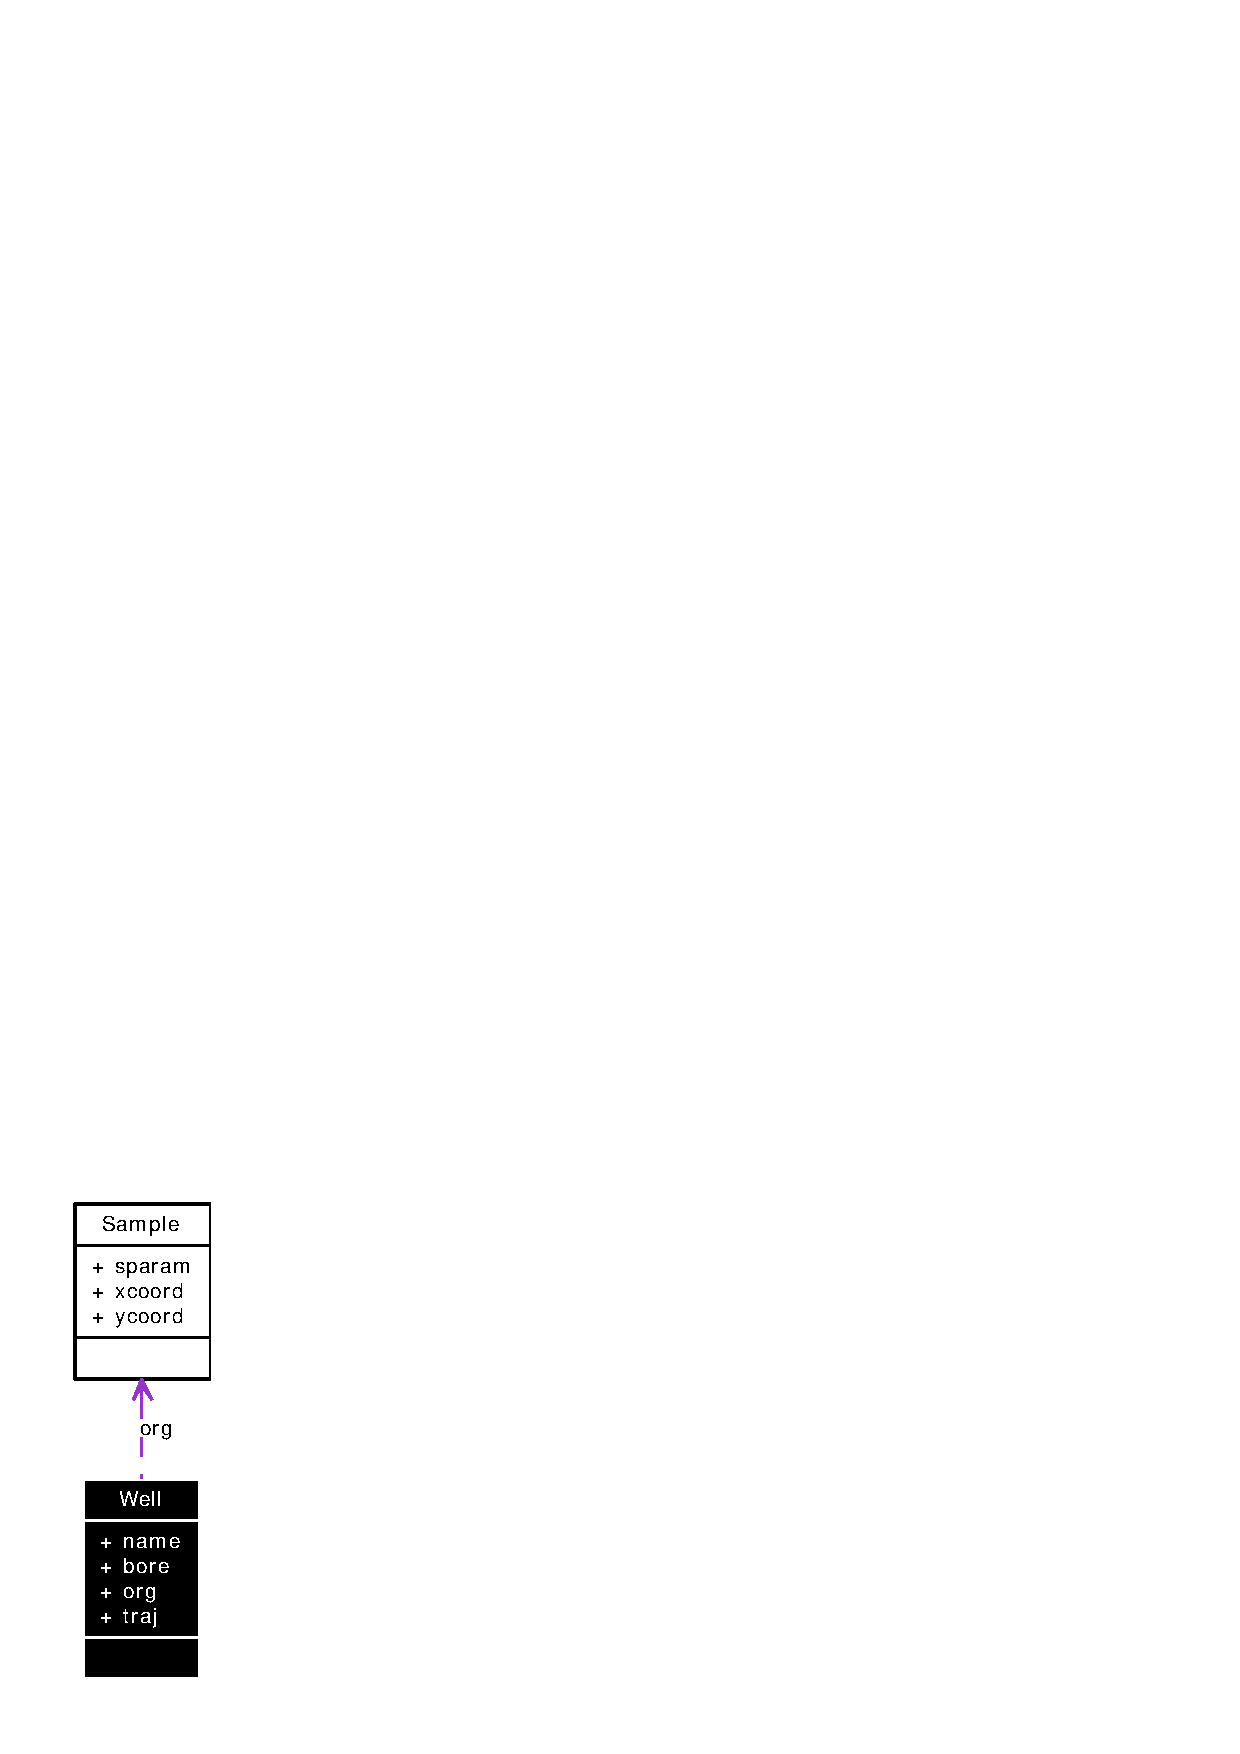
\includegraphics[width=50pt]{struct_well__coll__graph}
\end{center}
\end{figure}
\subsection*{Public Attributes}
\begin{CompactItemize}
\item 
char {\bf name} [32]\label{struct_well_o0}

\item 
long {\bf bore}\label{struct_well_o1}

\item 
{\bf Sample} {\bf org}\label{struct_well_o2}

\item 
Sample\_\-list {\bf traj}\label{struct_well_o3}

\end{CompactItemize}


\subsection{Detailed Description}




Definition at line 10 of file surface\_\-pick.h.

The documentation for this struct was generated from the following file:\begin{CompactItemize}
\item 
surface\_\-pick.h\end{CompactItemize}

\section{well\_\-grid Class Reference}
\label{classwell__grid}\index{well_grid@{well\_\-grid}}
\subsection*{Public Types}
\begin{CompactItemize}
\item 
typedef {\bf well\_\-grid\_\-key} {\bf key}\label{classwell__grid_w0}

\end{CompactItemize}
\subsection*{Public Member Functions}
\begin{CompactItemize}
\item 
double {\bf left} (int i) const \label{classwell__grid_a0}

\item 
double {\bf right} (int i) const \label{classwell__grid_a1}

\item 
double {\bf top} (int j) const \label{classwell__grid_a2}

\item 
double {\bf bottom} (int j) const \label{classwell__grid_a3}

\item 
double {\bf inf} (const {\bf well\_\-type} $\ast$w, int i, int j) const \label{classwell__grid_a4}

\item 
void {\bf populate} (const well\_\-graph \&g)\label{classwell__grid_a5}

\item 
{\bf well\_\-grid} (int cx, int cy, double x1, double x2, double y1, double y2)\label{classwell__grid_a6}

\item 
{\bf well\_\-grid} (int cx, int cy, double $\ast$init\_\-x, double $\ast$init\_\-y)\label{classwell__grid_a7}

\item 
{\bf $\sim$well\_\-grid} ()\label{classwell__grid_a8}

\end{CompactItemize}


\subsection{Detailed Description}




Definition at line 876 of file wellgrid.cpp.

The documentation for this class was generated from the following file:\begin{CompactItemize}
\item 
wellgrid.cpp\end{CompactItemize}

\section{well\_\-grid\_\-key Struct Reference}
\label{structwell__grid__key}\index{well_grid_key@{well\_\-grid\_\-key}}
Collaboration diagram for well\_\-grid\_\-key:\begin{figure}[H]
\begin{center}
\leavevmode
\includegraphics[width=60pt]{structwell__grid__key__coll__graph}
\end{center}
\end{figure}
\subsection*{Public Attributes}
\begin{CompactItemize}
\item 
int {\bf cell}\label{structwell__grid__key_o0}

\item 
const {\bf well\_\-type} $\ast$ {\bf well}\label{structwell__grid__key_o1}

\end{CompactItemize}


\subsection{Detailed Description}




Definition at line 857 of file wellgrid.cpp.

The documentation for this struct was generated from the following file:\begin{CompactItemize}
\item 
wellgrid.cpp\end{CompactItemize}

\section{well\_\-point\_\-set Class Reference}
\label{classwell__point__set}\index{well_point_set@{well\_\-point\_\-set}}
\subsection*{Public Types}
\begin{CompactItemize}
\item 
typedef wg\_\-split\_\-func {\bf split\_\-func}\label{classwell__point__set_w0}

\end{CompactItemize}
\subsection*{Public Member Functions}
\begin{CompactItemize}
\item 
void {\bf compute} (well\_\-graph \&, {\bf split\_\-func}, int ghost\_\-n, double ghost\_\-r)\label{classwell__point__set_a0}

\item 
void {\bf update} (const {\bf well\_\-type} $\ast$)\label{classwell__point__set_a1}

\item 
void {\bf remove} (const {\bf well\_\-type} $\ast$)\label{classwell__point__set_a2}

\item 
void {\bf clear} ()\label{classwell__point__set_a3}

\item 
leda\_\-list$<$ leda\_\-point $>$ {\bf c\_\-hull} () const \label{classwell__point__set_a4}

\item 
{\bf well\_\-point\_\-set} ()\label{classwell__point__set_a5}

\end{CompactItemize}


\subsection{Detailed Description}




Definition at line 47 of file wellgrid.cpp.

The documentation for this class was generated from the following file:\begin{CompactItemize}
\item 
wellgrid.cpp\end{CompactItemize}

\section{well\_\-type Struct Reference}
\label{structwell__type}\index{well_type@{well\_\-type}}
\subsection*{Public Attributes}
\begin{CompactItemize}
\item 
char {\bf name} [8]\label{structwell__type_o0}

\item 
float {\bf top\_\-x}\label{structwell__type_o1}

\item 
float {\bf top\_\-y}\label{structwell__type_o2}

\end{CompactItemize}


\subsection{Detailed Description}




Definition at line 105 of file wellgrid.h.

The documentation for this struct was generated from the following file:\begin{CompactItemize}
\item 
wellgrid.h\end{CompactItemize}

\section{wg\_\-wrapper Class Reference}
\label{classwg__wrapper}\index{wg_wrapper@{wg\_\-wrapper}}
Collaboration diagram for wg\_\-wrapper:\begin{figure}[H]
\begin{center}
\leavevmode
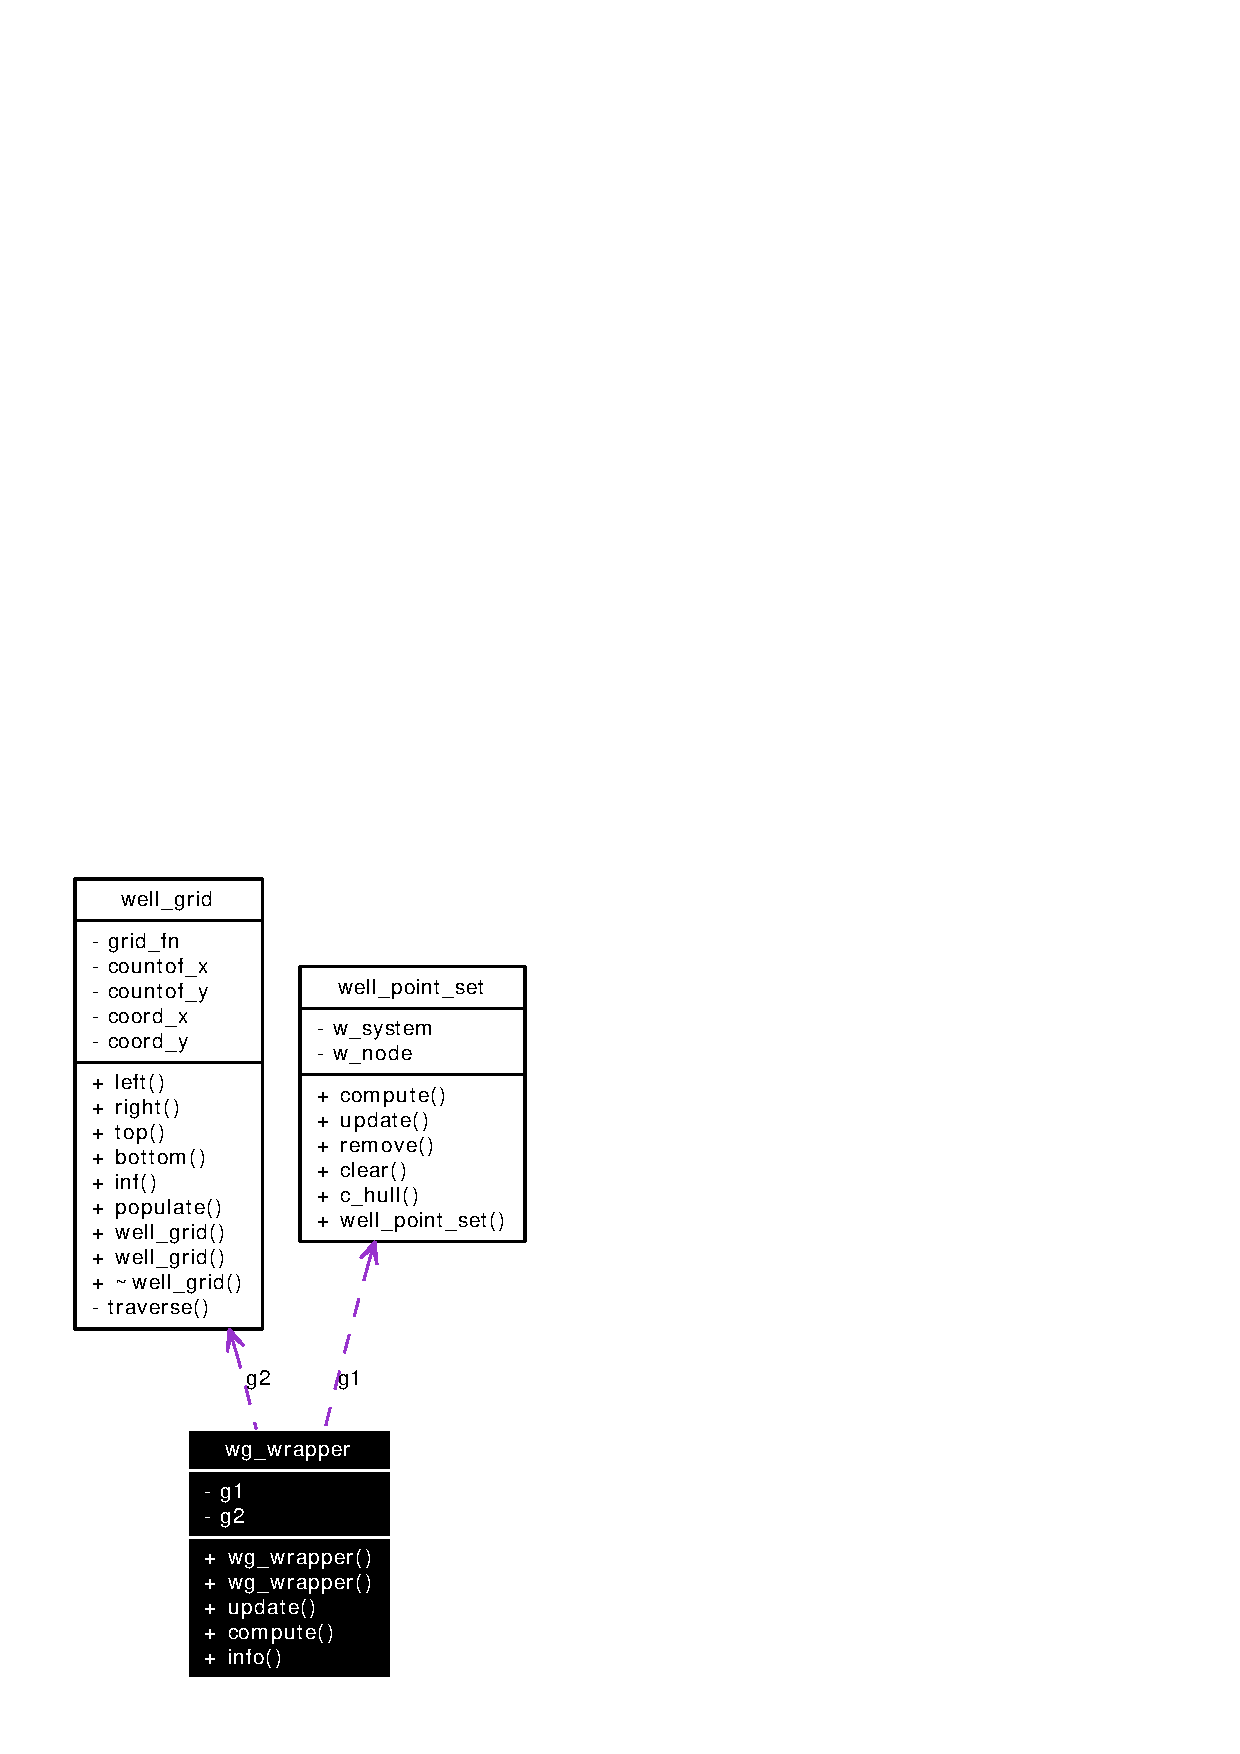
\includegraphics[width=126pt]{classwg__wrapper__coll__graph}
\end{center}
\end{figure}
\subsection*{Public Types}
\begin{CompactItemize}
\item 
typedef {\bf well\_\-point\_\-set::split\_\-func} {\bf split\_\-func}\label{classwg__wrapper_w0}

\end{CompactItemize}
\subsection*{Public Member Functions}
\begin{CompactItemize}
\item 
{\bf wg\_\-wrapper} (int cx, int cy, double x1, double x2, double y1, double y2)\label{classwg__wrapper_a0}

\item 
{\bf wg\_\-wrapper} (int cx, int cy, double $\ast$init\_\-x, double $\ast$init\_\-y)\label{classwg__wrapper_a1}

\item 
void {\bf update} (const {\bf well\_\-type} $\ast$w)\label{classwg__wrapper_a2}

\item 
void {\bf compute} ({\bf split\_\-func} fn)\label{classwg__wrapper_a3}

\item 
double {\bf info} (const {\bf well\_\-type} $\ast$w, int x, int y) const \label{classwg__wrapper_a4}

\end{CompactItemize}


\subsection{Detailed Description}




Definition at line 1051 of file wellgrid.cpp.

The documentation for this class was generated from the following file:\begin{CompactItemize}
\item 
wellgrid.cpp\end{CompactItemize}

\section{yyalloc Union Reference}
\label{unionyyalloc}\index{yyalloc@{yyalloc}}
\subsection*{Public Attributes}
\begin{CompactItemize}
\item 
short {\bf yyss}\label{unionyyalloc_o0}

\item 
YYSTYPE {\bf yyvs}\label{unionyyalloc_o1}

\end{CompactItemize}


\subsection{Detailed Description}




Definition at line 209 of file calc.tab.cpp.

The documentation for this union was generated from the following file:\begin{CompactItemize}
\item 
calc.tab.cpp\end{CompactItemize}

\section{Zero\_\-type Struct Reference}
\label{struct_zero__type}\index{Zero_type@{Zero\_\-type}}
\subsection*{Public Attributes}
\begin{CompactItemize}
\item 
int {\bf kind}\label{struct_zero__type_o0}

\item 
int {\bf start}\label{struct_zero__type_o1}

\item 
int {\bf final}\label{struct_zero__type_o2}

\item 
bool {\bf enter}\label{struct_zero__type_o3}

\end{CompactItemize}


\subsection{Detailed Description}




Definition at line 182 of file ps\_\-clip.cpp.

The documentation for this struct was generated from the following file:\begin{CompactItemize}
\item 
ps\_\-clip.cpp\end{CompactItemize}

\printindex
\end{document}
